%%%%%%%%%%%%%%%%%%%%%%%%%%%%%%%%%%%%%%%%%%%%%%%%%%%%%%%%%%%%%%%%%%%%%%%%%%%%%%%%
% University of Western Ontario Thesis Template
% By: Justin Quinn Veenstra, 2010
% With thanks to Mr. (soon to be Dr.) Will Robertson.


\documentclass[12pt,twoside]{report}
%% Decomment next line to use PostScript fonts
%%\UsePackage{times}
%%%%%%%%%%%%%%%%%%%%%%%%%%%%%%%%%%%%%%%%%%%%%%%%%%%%%%%%%%%%%%%%%%%%%%%%
%%                                                                    %%
%%                    ***   I M P O R T A N T   ***                   %%
%%                                                                    %%
%% Fill in the following fields with the required information:        %%
%%  - \department{...}  name of the graduate department               %%
%%  - \degree{...}      name of the degree obtained                   %%
%%  - \author{...}      name of the author                            %%
%%  - \title{...}       title of the thesis                           %%
%%  - \gyear{...}       year of graduation                            %%
%%  - \super{...}    supervisor
%%  - \firstname, \middlename, \lastname... there is additional documentation by the actual fields, so I'll leave it at that
%%%%%%%%%%%%%%%%%%%%%%%%%%%%%%%%%%%%%%%%%%%%%%%%%%%%%%%%%%%%%%%%%%%%%%%%
\usepackage{appendix}
\usepackage{graphicx}
\usepackage{amsmath}
\usepackage[byname]{smartref}
%\usepackage{hyperref} %comment out for hardcopy
\usepackage{txfonts}
\usepackage{tocloft}
\usepackage{amsmath}
\usepackage{amsfonts}
\usepackage{amssymb}
\usepackage{color}
\usepackage{booktabs}
\usepackage{longtable}
\usepackage{array}
\usepackage{multirow}
\usepackage{wrapfig}
\usepackage{float}
\usepackage{colortbl}
\usepackage{pdflscape}
\usepackage{tabu}
\usepackage{threeparttable}
\usepackage{threeparttablex}
\usepackage[normalem]{ulem}
\usepackage{makecell}
\usepackage{graphicx}
\usepackage{glossaries}
\usepackage{bm}
\usepackage{mathtools}
\usepackage{enumerate}
\usepackage{tikz}
\usetikzlibrary{arrows}
\usetikzlibrary{bayesnet}
\usepackage{caption}
\usepackage{url}
\usepackage{rotating}
\usepackage[noabbrev]{cleveref}
\usepackage[ruled,vlined]{algorithm2e}
\usepackage{xcolor}
\usepackage{setspace} 

\usepackage[colorinlistoftodos]{todonotes}
\usepackage{changes}

\newcommand{\Normal}{\operatorname{Normal}}
\newcommand{\Gmma}{\operatorname{Gamma}}
\newcommand{\Lognormal}{\operatorname{Lognormal}}
\newcommand{\needscite}{\colorbox{red}{Needs Citation}}

\makeatletter
\numberwithin{figure}{chapter}
\newenvironment{acknowledgements}%
{\clearemptydoublepage
	\begin{center}
		\section*{Acknowledgements}
	\end{center}
	\begingroup
}{\newpage\endgroup}

\newenvironment{dedication}%
{\clearemptydoublepage 
	\begin{center}
		\section*{Dedication}
	\end{center}
	\begingroup
}{\newpage\endgroup}

\newenvironment{preliminary}%
{\pagestyle{plain}\pagenumbering{roman}}%
{\pagenumbering{arabic}}

\addtoreflist{chapter}
\newtheorem{theorem}{Theorem}[section]
\newtheorem{lemma}[theorem]{Lemma}
\newtheorem{proposition}[theorem]{Proposition}
\newtheorem{corollary}[theorem]{Corollary}

\newenvironment{proof}[1][Proof]{\begin{trivlist}
		\item[\hskip \labelsep {\bfseries #1}]}{\end{trivlist}}
\newenvironment{definition}[1][Definition]{\begin{trivlist}
		\item[\hskip \labelsep {\bfseries #1}]}{\end{trivlist}}
\newenvironment{example}[1][Example]{\begin{trivlist}
		\item[\hskip \labelsep {\bfseries #1}]}{\end{trivlist}}
\newenvironment{remark}[1][Remark]{\begin{trivlist}
		\item[\hskip \labelsep {\bfseries #1}]}{\end{trivlist}}

\newcommand{\qed}{\nobreak \ifvmode \relax \else
	\ifdim\lastskip<1.5em \hskip-\lastskip
	\hskip1.5em plus0em minus0.5em \fi \nobreak
	\vrule height0.75em width0.5em depth0.25em\fi}

% Default values for title page.

%% To produce output with the desired line spacing, the argument of
%% \spacing should be multiplied by 5/6 = 0.8333, so that 1 1/2 spaced
%% corresponds to \spacing{1.5} and double spaced is \spacing{1.66}.
\def\normalspacing{1.25} % default line spacing


%% Define the "thesis" page style.
\if@twoside % If two-sided printing.
\def\ps@thesis{\let\@mkboth\markboth
	\def\@oddfoot{}
	\let\@evenfoot\@oddfoot
	\def\@oddhead{
		{\sc\rightmark} \hfil \rm\thepage
	}
	\def\@evenhead{
		\rm\thepage \hfil {\sc\leftmark}
	}
	\def\chaptermark##1{\markboth{\ifnum \c@secnumdepth >\m@ne
			Chapter\ \thechapter. \ \fi ##1}{}}
	\def\sectionmark##1{\markright{\ifnum \c@secnumdepth >\z@
			\thesection. \ \fi ##1}}}
\else % If one-sided printing.
\def\ps@thesis{\let\@mkboth\markboth
	\def\@oddfoot{}
	\def\@oddhead{
		{\sc\rightmark} \hfil \rm\thepage
	}
	\def\chaptermark##1{\markright{\ifnum \c@secnumdepth >\m@ne
			Chapter\ \thechapter. \ \fi ##1}}}
\fi

\pagestyle{thesis}
% Set up page layout.
\setlength{\textheight}{9in} % Height of the main body of the text
\setlength{\topmargin}{-.5in} % .5" margin on top of page
\setlength{\headsep}{.5in}  % space between header and top of body
\addtolength{\headsep}{-\headheight} % See The LaTeX Companion, p 85
\setlength{\footskip}{.5in}  % space between footer and bottom of body
\setlength{\textwidth}{6.25in} % width of the body of the text
\setlength{\oddsidemargin}{.25in} % 1.25" margin on the left for odd pages
\setlength{\evensidemargin}{0in} % 1.25"  margin on the right for even pages

% Marginal notes
\setlength{\marginparwidth}{.75in} % width of marginal notes
\setlength{\marginparsep}{.125in} % space between marginal notes and text

% Make each page fill up the entire page. comment this out if you
% prefer. 
\flushbottom

\setcounter{tocdepth}{1} % Number the subsubsections 
\def\normalspacing{1.25} % default line spacing

\newcommand\isco[1]{%
	\edef\@tempa{#1}%
	\def\@tempb{}%
	\ifx\@tempa\@tempb
	\else \\\underline{Co-Supervisor:}\vspace{0.35in}\\\dots\dots\dots\dots\dots\dots\dots\\{#1}\\
	\fi
}

\newcommand\isjoint[1]{%
	\edef\@tempa{#1}%
	\def\@tempb{}%
	\ifx\@tempa\@tempb
	\else \\\underline{Joint Supervisor:}\vspace{0.35in}\\\dots\dots\dots\dots\dots\dots\dots\\{#1}\\
	\fi
}

\newcommand\isalt[1]{%
	\edef\@tempa{#1}%
	\def\@tempb{}%
	\ifx\@tempa\@tempb
	\else \\\underline{Alternate Supervisor:}\vspace{0.35in}\\\dots\dots\dots\dots\dots\dots\dots\\{#1}\\
	\fi
}

\newcommand\isdefinedsig[1]{%
	\edef\@tempa{#1}%
	\def\@tempb{}%
	\ifx\@tempa\@tempb
	\else \\ \dots\dots\dots\dots\dots\dots\dots\\{#1}\\
	\fi
}
\newcommand\isdefinedspinetitle[1]{%
	\edef\@tempa{#1}%
	\def\@tempb{}%
	\ifx\@tempa\@tempb
	\else (Spine title: #1)\\
	\fi
}
\newcommand\coauthor[1]{%
	\edef\@tempa{#1}%
	\def\@tempb{}%
	\ifx\@tempa\@tempb
	\else \newpage \Large Co-Authorship Statement\normalsize\\\indent\\#1\\
	\fi
}

\newcommand\acknowlege[1]{%
	\edef\@tempa{#1}%
	\def\@tempb{}%
	\ifx\@tempa\@tempb
	\else \newpage \Large Acknowledgements\normalsize\\\indent\\#1\newpage
	\fi
}

%\renewcommand{\appendixtocname}{\Huge \textbf{List of Appendices} \normalsize}
\newcommand{\blank}{\hspace{-2mm}}
\newcommand{\super}{Dr. Daniel J. Lizotte} %supervisor
\newcommand{\superj}{} %joint supervisor, if there is one, leave blank if not (lbin)... only one of the three.
\newcommand{\superc}{} %co-supervisor, if there is one, leave blank if not (lbin)
\newcommand{\supera}{} %alternate supervisor, if there is one, leave blank if not (lbin)
\newcommand{\sco}{Committee Member 1}  %member of supervisory committee
\newcommand{\sct}{Committee Member 2}  %other member of supervisory committee (lbin)
\newcommand{\sch}{Committee Member 3}  %other member of supervisory committee (lbin)
\newcommand{\examo}{Examiner 1}  %examining committee (up to four, if less leave blank)
\newcommand{\examt}{Examiner 2}
\newcommand{\examth}{Examiner 3}
\newcommand{\examf}{}
\newcommand{\department}{Epidemiology and Biostatistics}
\newcommand{\degree}{Doctor of Philosophy}
\newcommand{\firstname}{Athanasios}
\newcommand{\middlename}{Demetrios}
\newcommand{\lastname}{Pananos}
%\renewcommand{\author}[1]{\ifx\empty#1\else\gdef\@author{#1}\fi} 
\newcommand{\authorname}{{\firstname} {\middlename} {\lastname}}
\newcommand{\titl}{Bayesian Pharmacokinetic Models for Inference and Optimal Sequential Decision Making with Applications in Personalized Medicine}
\newcommand{\spinetitle}{Bayesian Pharmacokientic Models with Applications in Personalized Medicine}%only if the above is more than 60 characters
\newcommand{\thesisformat}{Integrated Article} %or Integrated Article
\newcommand{\gyear}{\number\year}
\newcommand{\makecoauthor}{
	%Type information about coauthorship here/
	I would like to acknowlege my imaginary friend, Jummi for doing all the work. 
}
\newcommand{\makeacknowlege} {
	
	First, thank you to Dr.\ Dan Lizotte.  Dan has been an incredible mentor. So far as I can tell, Dan percieves me not as a trainee but as a colleague.  He has been patient, supportive, and kind.  I envy all future students who have the privellage to work with him.
	\newline
	\newline
	Thank you to my committe  for taking the time to read my thesis and provide edits to various components over the last 5 years.
	\newline
	\newline
	Thank you to Gary, who has been the best friend I have had. Our near daily statistical chats over coffee are something I look back on fondly.  For all the times we thought ``we should just quit'' -- and there were many -- I'm glad we didn't.
	\newline
	\newline
	Thank you to Dr.\ Simon Bonner, who I credit with cultivating the applied statistician I am today.  Much of my own statistical philosophy came from your Generalized Linear Models course.  It was a foundational course, in more ways than one, and represents a sort of line in the sand from which I started to call myself a statsitician propper.
}
\newcommand{\listappendixname}{List of Appendices}
\newlistof{myappendices}{app}{\listappendixname}
\newcommand{\myappendices}[1]{%
	\addcontentsline{app}{myappendices}{#1}\par}

\renewcommand{\maketitle}
{\begin{titlepage}
		\setcounter{page}{1}
		%% Set the line spacing to 1 for the title page.
		%\begin{spacing}{1} 
		\begin{large}
			\begin{center}
				\mbox{}
				\vfill
				{\MakeUppercase{\titl}}\\
				\isdefinedspinetitle{\spinetitle}
				(Thesis format: \thesisformat)\\
				\vfill
				by \\
				\vfill
				{\firstname} {\middlename} \underline{\lastname}\\
				\vfill
				Graduate Program in {\department}\\
				\vfill
				A thesis submitted in partial fulfillment\\
				of the requirements for the degree of\\
				\degree\\
				\vfill
				The School of Graduate and Postdoctoral Studies\\
				The University of Western Ontario\\
				London, Ontario, Canada\\
				\vfill
				{\copyright} {\authorname} {\gyear}  \\
				\vspace*{.2in}
			\end{center}
		\end{large}
		%   \end{spacing}
\end{titlepage}

}%\maketitle

\newcommand{\makecert}{
\setcounter{page}{2}
\vfill
\begin{center}
	\large
	THE UNIVERSITY OF WESTERN ONTARIO\\
	School of Graduate and Postdoctoral Studies\\
	\vfill
	\textbf{CERTIFICATE OF EXAMINATION}
\end{center}

\vfill
\begin{table}[ht]
	\begin{minipage}[t]{0.5\linewidth} %tabular instead?
		\begin{tabular}{l}
			\underline{Supervisor:}\vspace{0.35in}
			\isdefinedsig{\super}
			\isco{\superc}
			\isjoint{\superj}
			\isalt{\supera}
			\\
			\underline{Supervisory Committee:}\vspace{0.35in}
			\isdefinedsig{\sco}\vspace{0.15in}
			\isdefinedsig{\sct}\vspace{0.15in}
			\isdefinedsig{\sch}
		\end{tabular}
		\vfill
	\end{minipage}
	\hspace{0.5in}
	\begin{minipage}[t]{0.5\linewidth}
		\begin{tabular}{l}
			\underline{Examiners:} \\\vspace{.5cm}
			\isdefinedsig{\examo}\\
			\isdefinedsig{\examt}\\
			\isdefinedsig{\examth}\\
			\isdefinedsig{\examf}
		\end{tabular}
		\vfill
	\end{minipage}
	\vfill
\end{table}
\vfill
\begin{center}
	The thesis by \\ \vfill
	\textbf{\firstname{} \middlename{} \underline{\lastname}}\\
	\vfill
	entitled:\\\vfill
	\textbf{\titl}\\\vfill
	is accepted in partial fulfillment of the \\
	requirements for the degree of\\
	\degree\\
\end{center}
\begin{table}[ht]
	\begin{minipage}[t]{0.5\linewidth}
		\begin{tabular}{l}
			\dots\dots\dots\dots\dots\\
			Date
		\end{tabular}
	\end{minipage}
	\hspace{0.5in}
	\begin{minipage}[t]{0.5\linewidth}
		\begin{tabular}{l}
			\dots\dots\dots\dots\dots\dots\dots\dots\dots\dots\\
			Chair of the Thesis Examination Board
		\end{tabular}
	\end{minipage}
\end{table}

}

% Defined commands
\newcommand{\rhat}{\widehat{R}}


\makeatother
\begin{document}

%% ***   NOTE   ***
%% You should put all of your '\newcommand', '\newenvironment', and
%% '\newtheorem's (in other words, all the global definitions that you
%% will need throughout your thesis) in a separate file and use
%% "\input{filename}" to input it here.


%% This sets the page style and numbering for preliminary sections.
\begin{preliminary}
	
	%% This generates the title page from the information given above.
	\maketitle
	\addcontentsline{toc}{chapter}{Certificate of Examination}
	\makecert
	\newpage
	%\addcontentsline{toc}{chapter}{Co-Authorship Statement}
	%\coauthor{\makecoauthor}  %comment this out if none
	%\newpage
	\addcontentsline{toc}{chapter}{Acknowlegements}
	\acknowlege{\makeacknowlege}	%as above
	\addcontentsline{toc}{chapter}{Abstract}
	\Large\begin{center}\textbf{Abstract}\end{center}\normalsize
	%%  ***  Put your Abstract here.   ***
	%% (150 words for M.Sc. and 350 words for Ph.D.)
	
	Patients can react to a drug differently just by virtue of being different people, and this between-patient variability in drug response is an obstacle to optimal treatment.  Pharmacokinetic modelling offers one approach to studying drug response, often with covariate focused dose adjustment criteria being reported along side pharmacokinetic modelling.  However, excess variation in concentrations continues to be reported despite the use of these criteria, bringing into question optimal dosing strategies for some drugs.  This thesis provides methods for creating Bayesian pharmacokinetic models for two purposes: inference into the effects of covariates on concentrations and optimal sequential decision making for dose size.   The thesis addresses three objectives: To compare existing approaches to fitting Bayesian models with recent advancements in pursuit of fitting population pharmacokinetic models, to develop a framework for evaluating the benefits of collecting additional information for use in personalization, and to demonstrate how academic personalized medicine researchers can use all data available to them to study effects of clinical variables on pharmacokinetics. To this end, the thesis makes three research contributions. First, a simulation study demonstrating that inferences using popular inference methods in pharmacokinetic research can lead to different and poorer calibrated decisions as compared to newer inference methods.  The model presented in the simulation study was developed using a specific parameterization achieved through non-dimensionalization of the differential equation governing the mass transit of the drug and enables more reliable inference by sampling using Hamiltonian Monte Carlo as compared to a standard parameterization. Second, a unified framework for the development and simulation based evaluation of personalization based on pharmacokinetic modelling combined with dynamic treatment regimes. Lastly, a demonstration of how investigators can fit Bayesian pharmacokinetic models with the aim of accurate modelling of pharmacokinetics and exploration of novel variables using data from heterogeneous sources.  These contributions provide methodologies do address two central goals of personalized medicine -- identification of factors driving between patient variability in drug response, and selection of an optimal dose --  and can enable a richer set of personalized decisions to be made.
	
	\vfill
	\textbf{Keywords:} Bayesian Statistics, Pharmacokinetics, Hierarchical Model, Personalized Medicine
	\newpage
	\tableofcontents\newpage
	\newpage
	\addcontentsline{toc}{chapter}{List of Figures}
	\listoffigures
	\newpage
	\addcontentsline{toc}{chapter}{List of Tables}
	\listoftables\newpage
%	\addcontentsline{toc}{chapter}{List of Appendices}
%	\listofmyappendices\newpage
	%\addcontentsline{toc}{chapter}{List of Abbreviations, Symbols, and Nomenclature}
	%\large List of Abbreviations, Symbols, and Nomenclature \normalsize
	%\newpage
\end{preliminary}
%% End of the preliminary sections: reset page style and numbering.

%%%%%%%%%%%%%%%%%%%%%%%%%%%%%%%%%%%%%%%%%%%%%%%%%%%%%%%%%%%%%%%%%%%%%%%%
%%                                                                    %%
%%                    ***   I M P O R T A N T   ***                   %%
%%                                                                    %%
%% Put your Chapters here; the easiest way to do this is to keep each %%
%% chapter in a separate file and \include all the files right here.  %%
%% Note that each chapter file should start with the line             %%
%% "\chapter{ChapterName}".  Note that using "\include" instead of    %%
%% "\input" makes each chapter start on a new page.                   %%
%%%%%%%%%%%%%%%%%%%%%%%%%%%%%%%%%%%%%%%%%%%%%%%%%%%%%%%%%%%%%%%%%%%%%%%%
% As an example...

\doublespacing
\chapter{Introduction}

\section{Motivation}

Different patients can react to a drug differently just by virtue of being different people, even when said patients match on clinical variables.  This between-patient variability in drug response is an obstacle to optimal treatment since some patients may experience heightened response (possibly leading toxicity) while others may experience lowered response (possibly leading to weakened response or inefficacy).  Personalized medicine is a response to this variation, with the goals of: 1) identifying drugs for which between-patient variation is a key issue for effective treatment,  2) to address/identify factors driving this variation, 3) to treat the right patient with the right drug  of the right amount at the right time, 4) and to aid in the prevention of adverse events associated with said drugs \cite{morse2015personalized}.  This thesis is primarily concerned with goals of identifying which factors are drivers of between patient variability in service of better selecting the right dose for the right patient, and is thus aligned with goals 2 and 3.

The setting of interest for this thesis is pharmacokinetics, which concerns itself with the time course of drug concentrations in the body \cite{ rosenbaum2016basic}.
Effective drug response requires adequate systematic exposure.  Since drug concentration is a means of measuring drug exposure,  an understanding which factors drive variation in concentration can give insight into factors driving variation in response.  To this end, many pharmacokinetic modelling studies seek to identify clinical, genetic, and lifestyle factors which are associated with changes in concentration \needscite. Some studies provide dose adjustment criteria.  As an example \todo[inline]{place apixaban dose adjustment criteria for one of those papers?}.  These recommendations are personalized in so far as they identify sub-populations of patients which may see predictably larger/smaller concentrations as a function of standard doses, however for some drugs additional concentration variability beyond that observed in clinical trials is being observed \needscite, raising questions about optimal dosing for these drugs.  The discovery of this excess variation in applied settings motivates the ``fine tuning'' of the pharmacokinetic modelling done in previous studies for application in the population of interest.


This thesis outlines methods for creating Bayesian pharmacokinetic models for two purposes: inference into the effects of covariates on pharmacokinetic parameters and thereby concentrations, as well as use for these models in sequential decisions on dose size.    Bayesian statistics is the formalism adopted so as to incorporate and directly build upon prior information from other pharmacokinetic modelling efforts.These models are an attempt to address questions pertaining to the second goal of personalized medicine, identification of factors driving variation in drug response.  The models will be directly incorporated into a sequential decision making framework thereby addressing questions pertaining to the third goal of personalized medicine, optimal dosing.


% Why do we need personalized medicine?
% There is unexplained variation in drug response.  This can be a hurdle for optimal treatment because excess variation means some people have increased response potentially leading to toxicity, while others have decresed response, possibly leading to inefficacy.

% What is personalized medicine trying to accomplish/
% 1) Find drugs with large response variability, 2) discover factors associated with this variability, 3) find right drug right time, 4) prevent adverse events.

% What is this thesis aiming to accomplish?
% Work towards goals 2 and 3.

% How are we going to do that and why that way?
% Use pharmacokinetics.  Effective drug response requires adequate  systematic exposure.  Since concentration is a means of measuring exposure, drivers of concentration can give insight into variability in response.

% Ok cool, what is this thesis going to do in that realm?
% Many PK studies already look at factors associated with variation in concentration.  The results of these studies are personalized in so far as we identify some patients which need adjustment, but we're seeing more variation than expexted which raises questions about optimal dosing strategy.

% Ok, so there is additional variability.  Whats the gap?
% 




\section{Objectives}

I address three objectives motivated by the desire to identify sources of between patient variability and account for these in downstream decisions on drug dosing:

\begin{enumerate}[1)]
	\item To contrast existing approaches to fitting Bayesian models with recent advancements in the pursuit of fitting population pharmacokinetic models for use in decision making problems in determination of dose size to achieve a desired risk level.
	
	\item To develop a framework to evaluate the  benefits of collecting additional information on patients to use in pharmacokinetic models for personalization against the additional burden posed on the patient to adhere to additional requirements.
	
	\item To demonstrate how personalized medicine researchers in academic centres can use all data available to them, even if those data do not come from tightly controlled studies, to study effects of clinical variables on pharmacokinetics while also exploring new variables which may explain additional variation.
\end{enumerate}


\section{Research Contributions}

\section{Thesis Organization}

This thesis is written with an integrated-article format.  \textbf{Chapter 2} provides necessary background on  concepts and terms that are needed to understand the body of the work.  \textbf{Chapter 3} provides a literature review of recent advances in the fields of Bayesian statistics, sequential decision making, and pharmacokinetics, providing context for the three articles to follow.  \textbf{Chapters 4, 5, and 6} include the integrated articles which address objective 1 --- 3 respectively.  \textbf{Chapter 7} concludes the thesis with an overarching discussion and examines possible subsequent areas of investigation.  Any \textbf{appendices} are included at the end of each integrated article, and may contain supporting materials such as extra information on methods, additional exposition for models, and additional visualizations.  Due to the nature of the integrated article format, there is some repetition between introductory sessions.		
\chapter{Background}

In this chapter, I describe the necessary background for the research presented in this thesis.  The focus of the first section is differential equations, specifically first order separable equations and the Laplace Transform.  I briefly discuss conditions under which a differential equation has a unique solution, as well as techniques for qualitative analysis of a system's dynamics under famalies of eqivalent parameterizations.  Then, I discuss Bayesian statistics, touching on model design, model checking, and model fitting.  In the next section I discuss population pharmacokinetic models, touching on their derivation through differential equations as well as extensions to include multiple doses.  I conclude this chapter with a treatment of dynamic treatment regimes and estimation of an optimal policy through Q learning.

\section{Differential Equations}\label{sec:ODE}

\subsection{Initial Value Problems, Existence, and Uniqueness}

A differential equation is an equation which relates the derivative of an unknown function $y(t)$ to a known function $f(t, y(t), \theta)$. Here, the function $f$ may depend on parameters, $\theta$ which can be known exactly or require estimation from data. For economy of thought, dependence of $f$ on $\theta$ is implied though not always explicitly stated. A differential equation is called \textit{ordinary} (refereed to as an \textit{ODE}) if $y$ is a function of a single scalar variable $t$, which for the purposes of this thesis can be considered to be time. An ODE together with an \textit{initial condition} -- a value of $y$ at some point $t_0$ in its domain --  is refereed to as an \textit{initial value problem} (or sometimes an \textit{IVP}), 

\begin{equation}\label{IVP}
	\dfrac{dy(t)}{dt} = f(t, y(t), \theta) \quad y(t_0) = y_0
\end{equation}

\noindent If the function $f$ can be written as $f(t, y(t)) = Q(t) - I(t) y(t)$, then we call the ODE a \textit{first order linear ordinary differential equation}.  The equation is called first order because the highest order derivative is of order one, and the linear because the equation is a linear function of the derivative. 

Not every IVP which can be written down has a solution, but there do exist general criteria for existence and uniqueness to a solution for \cref{IVP}.  The only requirements are that a) $f$ be continuous in $t$, and b) $f$ be Lipschitz continuous in $y$.  Under these conditions, Picard–Lindelöf theorem \cite{morris1963ordinary}.

\begin{theorem}[\emph{Picard–Lindelöf Theorem}]
	Let $D \subseteq \mathbb{R} \times \mathbb{R}^n$ be a closed rectangle with $(t_0, y_0) \in D$, and let $f : D \to \mathbb{R}^n$ be a function that is continuous in $t$ and Lipschitz continuous in $y$.  Then, there exists some $\epsilon>0$ such that \cref{IVP} has a unique solution $y(t)$ in an interval centred at $t_0$ with radius $epsilon$.
\end{theorem}

\noindent This thesis is mainly concerned with functions which are continuous in $y$.  If a function is continuous in a variable, then it is also Lipschitz continuous.  Hence, all IVPs for which we concern ourselves with have a unique solution.


\subsection{Solutions to First Order Linear Equations}

So long as the function $f(t, y(t)) = Q(t) - I(t) y(t)$ satisfies the conditions for the Picard–Lindelöf theorem, then a solution exists and it is unique.  Assuming $Q(t)$ and $I(t)$ are written in terms of analytic functions, then the solution to \cref{IVP} can be written out analytically.  Let $P(t) = \exp(\int I(t) \, dt)$ be an \textit{integrating factor}.  Multiplying both sides of the ODE by $P(t)$ yields

\begin{align}
	\dfrac{dy}{dt} + I(t)y(t) &= Q(t) \\
	P(t)\dfrac{dy}{dt} + P(t)I(t)y(t) &= P(t)Q(t) 
\end{align}

\noindent  The form of $P(t)$ implies $P'(t) = P(t)I(t)$,and so the left hand side of the differential equation looks as if it is the result of the product rule

\begin{align}
 \dfrac{d}{dt} \Big( P(t)y(t) \Big) &= P(t)\dfrac{dy}{dt} + P(t)I(t)y(t) \\
														  &= P(t) Q(t)
\end{align}

\noindent Integrating and division by $P(t)$ (which is possible since $P(t)>0$ by construction) yields the solution to the differential equation

\begin{equation}
	y(t) = \dfrac{\int Q(t) P(t)\, dt}{P(t)}
\end{equation}

\noindent Wherein the constant of integration from the numerator is determined by using the initial condition. Our general takeaway is that so long as $f$ satisfies the conditions s for the Picard–Lindelöf theorem, and $Q(t)$ and $I(t)$ are not sufficiently complicated so as to prevent integration, then the solution to \cref{IVP} can be written down exactly.


\subsection{Non-dimensionalization}

Differential equations representing physical systems can often have several parameters, and the qualitative behavour for the solution can be similar across many different families of differential equations. A technique used by applied mathematicians to study the qualitative behavour of a differential equation is known as \textit{non-dimensionalization}.  The technique involves rescaling the solution $y(t)$ (which could have a variety of units depending on what is being modelled) and the time variable $t$ (which could be measured in seconds, hours, minutes, etc.) to be unitless. Let $a \neq 0$ be measured in the same units as $t$ and let $b \neq 0$ be measured in the same units as $y$.  Then, we can define non-dimensional variables as $t = a \tau $ and $y = b x)$.  The non-dimensionalization of the differential equation $dy/dt = f(t, y(t))$  in terms of $\tau$ and $x$ is obtained by applications of differention rules

\begin{align}
	\dfrac{d }{dt} \Big( y(t) \Big) &=  	\dfrac{d }{dt} \Big( b x(\tau) \Big)\\
													&= b \dfrac{dx(\tau) }{d\tau} \dfrac{d \tau}{dt}\\
													&= \dfrac{b}{a} \dfrac{dx(\tau)}{d\tau}
\end{align}


\noindent which yields $dx / d \tau = a/b f(a\tau, bx(\tau))$.  The approach is similar to normalization in statistics (e.g. subtracting the mean and dividing by the standard deviation).  The re-scaling allows one to examine families of solutions for which $a/b$ is constant, giving insight into the characteristic dynamics of the system. 


\subsection{The Laplace Transform and Forcing Functions}

Under the conditions that a function $f$ is piecewise continuous on an interval $0 \leq t \leq A$ for any positive $A$, and that $\vert f(t) \vert \leq K \exp(at)$ when $M \leq t$ for real constants $0< K, a, M $, then the integral

$$ \int_0^\infty f(t) e^{-st} \, dt  $$ 

\noindent exists and is called \textit{The Laplace Transform}, denoted $\mathcal{L}\left\{f\right\}(s)$.  The Laplace Transform can be used to turn a first order linear differential equation into an algebraic equation due to the property that  $\mathcal{L}\left\{f'\right\}(s) = s\mathcal{L}\left\{f\right\}(s) - f(0) $, which can be demonstrated by applying integration by parts. The algebraic equation can then be solved and inverted from $s$ space to $t$ space.  The Laplace Transform can be used to solve differential equations with discontinuous forcing functions.  These differential equations take the form 

\begin{equation}
	\dfrac{dy}{dt} + I(t)y(t) = Q_1(t) + H(t)Q_2(t) \>.
\end{equation}

\noindent Here, $H(t)$ is a Heaviside step function

\begin{equation}
	H(t) = \begin{cases}  1 & t>0 \\ 0 & \mbox{else} \end{cases}
\end{equation}

\noindent  When $t<0$,  $Q_2(t)$ is essentially ``turned off'' and its effect on the dynamics of $y$ is 0.  When $t>0$, the effect is then ``turned on''. As an example, we consider a differential equation which will be of great use in the remainder of this thesis

\begin{equation}
	\dfrac{dy}{dt} + \alpha y(t) = \exp(-t)  + H(t - t_1) \exp(-(t - t_1)) \quad y(0) = 0 \>.
\end{equation}

\noindent Here, the dynamics undergo a force of $\exp(-(t-t_1))$ when $0<t_1 \leq t$.  The Laplace Transform can be used on both sides (leveraging tables of Laplace Transforms for common functions \cite{boyce2021elementary}) of the differential equation to yield

$$ s\mathcal{L}\left\{y\right\}(s) - y(0) + \alpha \mathcal{L}\left\{y\right\}(s) = \dfrac{1 + \exp(-st_1)}{1+s} \>.  $$

\noindent The equation is now algebraic in terms of $\mathcal{L}\left\{y\right\}(s)$.  Solving for $\mathcal{L}\left\{y\right\}(s)$ yields

\begin{equation}
	\mathcal{L}\left\{y\right\}(s) =  \dfrac{1 + \exp(-st_1)}{1+s} \dfrac{1}{s+\alpha} \>,
\end{equation}

\noindent and applying the inverse Laplace Transform yields

\begin{equation}
	y(t) = \dfrac{\Big(\exp(-t) - \exp(-\alpha t)\Big) + H(t-t_1)\Big(\exp(-(t-t_1)) - \exp(-\alpha(t-t_1))\Big)}{\alpha-1}
\end{equation}

\noindent  Readers may note that because the two forcing functions in the differential equation were identical (one was just shifted $t_1$ units to the right) the solution to the differential equation is comprised of the same two functions, one of which is shifted $t_1$ units to the right.  The Laplace Transform will be of particular use when deriving solutions to differential equations which describe mass transit of a drug through the blood.  In these applications, multiple doses are taken through time and can be represented as discontinuous forcing functions using Heaviside functions.  When takes a dose of a drug, the effect of that dose on the system dynamics is ``turned on'' at the time of ingestion. Additionally, because the Laplace Transform is a linear operator, we can consider arbitrarily many discontinuous forcing functions, to which I have limited my exposition to one for economy of thought.
\section{Bayesian Statistics}

In this section, I introduce some key concepts of Bayesian statistics to be used in the remainder of the thesis.  I begin by briefly reviewing how Bayesianism differs from Frequentism in philosophy.  I then introduce Bayes nets as a tool for visualizing the factorization of the joint distribution.  Finally, I discuss model diagnostics and MCMC computation for Bayesian inference.


\subsection{The Bayesian Philosophy on Probability}
%\todo[inline]{This is a can of worms. Re-frame this paragraph by saying what specific other people say about this issue and citing. "So-and-so characterises frequentism as (cite). "Gelman charcterises the Bayesian approach as (cite). Jaynes is right out." Or, "Many researchers describe Bayesian approach as subjective (citecitecite)." }


Gelman and colleagues have described Frequentist interpretations of probability as the `` relative frequency obtained in a long sequence of [events], assumed to be performed in an identical manner, physically independent of one another ''   \cite[p.~12]{gelman2013bayesian}.   Frequentism has been contrasted against Bayesianism, which has sometimes been said to view probability as a subjective form of uncertainty quantification \cite{gelman2013bayesian}.

Core to Bayesian statistics is Bayes' rule \cite[p.~7]{gelman2013bayesian}

\begin{equation}\label{Bayes}
	p( \bm{\theta} \vert y) \propto p(y \vert \bm{\theta}) p(\bm{\theta}) \>.
\end{equation}

\noindent  Here, $ \bm{\theta} $  and $y$ can refer to events (e.g. $p(\bm{\theta} \vert y)$ could refer to the probability of having a disease given you test positive), but in the remainder of this thesis $\bm{\theta}$ will refer to model parameters, and $ y $ to observed data.  The distributions $ p( \bm{\theta} \vert y) $, $ p(y \vert \bm{\theta}) $, and $p(\bm{\theta})$ are referred to as the \textit{posterior}, \textit{the likelihood}, and \textit{the prior} respectively.  Since the product of Bayes' rule is a probability distribution (i.e. the probability of the parameters conditioned on the data), inferences resulting from a Bayesian analysis are expressed in probabilistic statements. Bayesian modelling begins by specifying a full probability model for the phenomenon.  A likelihood for the data generating process is specified, and prior knowledge about the parameters is codified in terms of a probability distribution (i.e.\ the prior).  Conditioning on the observed data is performed, and the posterior is calculated and interpreted.  Finally, the resulting model is evaluated and the implications of the resulting posterior are assessed.  

\subsection{Bayesian Networks}



Bayesian models describe the full joint distribution over all variables and parameters of interest, and can become quite complex. Bayesian networks (Bayes nets) can be used to simplify model description by dividing the model into components and then describing the relationships between those components. A Bayes net is a directed acyclic graph which represents a factorization of the joint probability distribution of the model. The nodes of the graph denote random variables (which include parameters), while the edges denote dependence of the child node on the parent node \cite{Bishop2006pattern}. 

Shown in \cref{bayesnet} is an example of a Bayes net for Gelman's rat tumour example in \cite{gelman2013bayesian}.  A total of $ N = 71 $ experiments on lab rats have been conducted in the past to assess the risk of developing endometrial stromyl polyps.  A rat can either develop the endometrial stromal polyp, or not develop the endometrial stromyl polyp, so the number of rats which develop the polyp, $ y_i $, is modelled as binomial.  Each of the 71 previous experiments is modelled as having it's own risk of developing the polyp, $ \theta_i $, which we postulate are drawn from a beta distribution with parameters $ \alpha $ and $ \beta $.  

Algebraically, the model would be written as 
%
\begin{align*}
	[\alpha,\beta]^T &\sim p(\alpha, \beta) \\
	\theta_i \vert \alpha, \beta &\sim \operatorname{Beta}(\alpha,\beta) \quad i = 1 \dots N\\
	y_i \vert \theta_i, \alpha, \beta &\sim \operatorname{Binomial}(\theta_i ; n_i) \quad i = 1 \dots N
	\end{align*}
%
Here, $ p(\alpha, \beta)  $ is the prior for the parameters of the beta distribution, and $ n_i $ is the number of rats in the $ i^{th} $ experiment.  This same model is written as a Bayes net in \cref{bayesnet}.   The node containing $ \alpha $ and $ \beta $ is the parent of $ \theta $, indicating that $ \theta $ depends on $ \alpha $ and $ \beta $, and $ y $ is the child of $ \theta $, indicating that $ y $ depends on $ \theta $. It is worth noting that if the parent nodes are known, then the child nodes are independent of all other nodes in the model. The rectangle surrounding $ \theta $ and $ y $ signifies that there are $ N $ such copies of these random variables which are considered exchangeable conditioned on the parent nodes.  Instead of explicitly writing out all $ N=71 $ of these random variables, we instead place them in what is known as a ``plate", and indicate in the bottom corner how many replicates there are.  Bayes nets make it very easy to write out the posterior distribution of the parameters.  We simply follow the net from the bottom up, conditioning each node on it's parent nodes.  The posterior for this model is then

 \[ p(\alpha,\beta, \theta \vert y) \propto p(\alpha,\beta) \prod_{i = 1}^N p(\theta_i \vert \alpha, \beta) p(y_i\vert \theta_i)  \]

\begin{figure}[h!]

	\centering
	\begin{tikzpicture}
		\node[latent] (ab) {$\alpha,\beta$};
		\node[latent, below = of ab]  (theta) {$\theta$};
		\node[obs, below = of theta](y){$y$};
		
		\edge{ab}{theta};
		\edge{theta}{y};
		
		\plate{exp}{(theta)(y)}{$N$};
	\end{tikzpicture}
	\caption[Hierarchical binomial model bayes net]{Bayes net for hierarchical binomial model.  Note here that nodes with shading correspond to observed data, while nodes without shading are latent, or unobserved.}
	\label{bayesnet}
\end{figure}

\noindent Note that while the Bayes net describes the dependence structure of the model, it does not specify the forms of the individual conditional distributions; these must also be provided to fully specify the model.

\subsection{Model Assessment}

Once a model is specified, and the posterior for the parameters obtained, the model fit, not only to the data but also to the practitioner's substantive knowledge, must be assessed.  

Since the result of a Bayesian analysis is the posterior distribution over the model parameters given the observed data, data can be simulated from the inferred data generating process.  Let $ y $ be observed data, and $ \theta $ be a vector of parameters for the model.  Denote $ \tilde{y} $ as replicated data from the data generating process, or as Gelman writes, ``data that we \textit{would} have seen tomorrow if the experiment that generated $ y $ today were replicated with the same model and the same value of $ \theta $ that produced the observed data" \cite[page~145]{gelman2013bayesian}.  Then the distribution of the replicated data conditioned on the observed data is 
%
\begin{equation}\label{PPD}
	p(\tilde{y} \vert y) = \int p(\tilde{y} \vert \bm{\theta}) p(\bm{\theta} \vert y) \, d\bm{\theta}  \>.
\end{equation}
%
The distribution in \cref{PPD} is called the \textit{posterior predictive distribution}.  If the model fits the data well, then observed data should look plausible under the posterior predictive distribution. In a posterior predictive check, simulated data sets are generated from \cref{PPD} and are compared to the observed data.  Any systematic differences between observed and simulated may point to areas in which the model can be improved.

\subsection{Maximum A Posteriori (MAP) and The Laplace Approximation to the Posterior}

The integrals in Bayesian statistics required to evaluate probabilities quickly become intractable even when considering simple models. Point estimates for model parameters can be obtained by maximizing the log posterior density.  If the posterior is $p(\bm{\theta} \vert y)$, then a point estimate for $\bm{\theta}$ is

\begin{align}
	\bm{\theta}_{\text{MAP}} &= \underset{\bm{\theta} \in \mathbb{R}^p}{\arg\max} \Big\{ \log p(\bm{\theta} \vert y) \Big\} \nonumber \\ 
	& = \underset{\bm{\theta} \in \mathbb{R}^p}{\arg\max} \Big\{\log p(y \vert \bm{\theta}) + \log p(\bm{\theta}) \Big\}  \nonumber
\end{align}

\noindent This approach is known as \textit{Maximum A Posteriori} or MAP for short \cite{murphy2012machine}.  The point estimate  $\bm{\theta}_{\text{MAP}} $ corresponds to the mode of the posterior distribution.  If the prior $p(\bm{\theta})$ places uniform probability over all values of $\bm{\theta}$ then the MAP estimate corresponds to the maximum likelihood estimate.  When the prior  is not uniform over $\bm{\theta}$, then the prior acts as a regularizing term on the maximum likelihood estimate, with more informative priors offering more regularization.

The MAP estimate is attractive because of its speed (as compared to other forms of estimation for Bayesian models discussed below).  However, it is only a point estimate rather than a distribution.  To further approximate the posterior distribution, a Laplace Approximation to the posterior can be made by performing a quadratic approximation to the log posterior density \cite{murphy2012machine}.  The result of this technique is that the posterior is locally modelled as Gaussian

$$ p(\bm{\theta} \vert y)  \approx \Normal(\bm{\theta}_{\text{MAP}}, \Lambda^{-1}) \>. $$

\noindent Here, $\Lambda$ is the estimated precision matrix, obtained by computing the Hessian of the negative log posterior at the MAP estimate.


\subsection{Markov Chain Monte Carlo \& Modern Methods}

Computational methods have been developed that can sample from the posterior distribution without having to know the exact analytical form of the posterior distribution. The suit of computational methods for sampling from the posterior are called \textit{Markov Chain Monte Carlo} (MCMC) methods.  These methods simulate Markov chains whose limiting distribution is the posterior distribution \cite{livingstone2016geometric}.  The earliest MCMC methods for drawing  samples from the posterior are The Metropolis-Hastings Algorithm and Gibbs Sampling \cite{gelman2013bayesian,mcelreath2016statistical}.  Recently however, these algorithms have given way to more efficient algorithms, known as \textit{Hamiltonian Monte Carlo} (HMC) methods.  In these methods, the posterior is idealized as a high dimensional surface in the model's parameter space on which a particle of mass $ m $ rolls after being given a random position and momentum.  The geometry of the surface influences the movement of the particle, and thus influences the samples obtained.   The theory for HMC is quite dense and so  I refer interested readers to the following resources \cite{ gelman2013bayesian, livingstone2016geometric, mcelreath2016statistical,neal2011mcmc, hoffman2014no,betancourt2017conceptual} for further explanation.  Because of HMC's complexity and requisite background theory on Hamilonian dynamics and measure theory, I will consider HMC a black box for the purposes of this thesis.

All of these sampling methods result in a user specified number of sequences of samples of size $ M$, often simply referred to as \textit{chains}. After obtaining $ M $ samples, and preferably omitting the first $ K $, the remaining $ M-K $ samples are treated as \textit{iid} draws from the posterior distribution.  The chains can then be used to estimate expectations of model parameters, uncertainty in those estimates, and make predictions.

\subsection{Diagnostics for Hamiltonian Monte Carlo}

%Under certain conditions, a law of large numbers and a central limit theorem exists for these Markov chains \cite{livingstone2016geometric, betancourt2017robust}, allowing users to be confident in inferences made from the samples obtained.  General conditions under which a chain is and is not geometrically ergodic exist \cite{livingstone2016geometric}, however these properties can be assessed via diagnostics on the Markov chains themselves.

In MCMC and HMC, several chains are usually initialized and allowed to run for sufficiently long to as to (hopefully) arrive at their stationary distribution.  If geometric ergodicity holds, then all chains should arrive at the same stationary distribution, and thus be exploring the same space.  The Gelman-Rubin diagnostic  measures how well the chains are exploring the space by comparing the within chain variance to the between chain variance \cite{gelman2013bayesian}.  In practice, $ 1.05<\rhat $ indicates a problem with the chains, and inference should not be made from the samples drawn \cite{betancourt2017robust}.

Another diagnostic is the effective sample size, $ n_{\mathit{eff}} $.  Theories of convergence of functions of random variables that assume independence are inappropriate as the samples from the Markov chains are correlated.  Effective sample size is a heuristic used to measure how close the samples are to being independent.  Effective sample size is defined as
%
\[ n_{\mathit{eff}} = \dfrac{M-K}{1+ 2\displaystyle\sum_k \rho(k)} \>. \]
%
Here $ M-K $ is the length of the chain and $ \rho(k) $ is the lag-$k$ within chain correlation \cite{gelman2013bayesian,kass1998markov}.  If the chains are autocorrelated, then $n_{\mathit{eff}} <M-K$, and if the chains are completely independent $n_{\mathit{eff}} = M-K$. If chains are highly correlated, then $n_{\mathit{eff}} \ll M-K$, and inferences made from the samples should be avoided because of the bias the correlation would impart.
\section{Pharmacokinetics} \label{PKPD}

In this section, I introduce the central pharmacokinetic model used in this research.  I derive the model from a differential equation and examine its qualitative behavour using non-dimensionalization.  Population pharmacokinetic models are discussed as a generalization of the one compartment pharmacokinetic model


\subsection{A One Compartment Pharmacokinetic Model} 

To analyze the time course of drug mass in various parts of the body, compartmental models may be used.  These models posit that the body (or relevant organs/systems of the body) is comprised of compartments from which drug can flow in and out. The rates at which the drug can enter and exit each compartment are specified, and a differential equation for each compartment can be written down and solved using methods outlined in \cref{sec:ODE}.

An example of these models used for orally-administered drugs is the one--compartment pharmacokinetic model with first order elimination.  The model posits the following \cite{wakefield1992bayesian}:  
%
\begin{itemize}
\item The rate of drug absorption from the gut ($ G  $) into the blood plasma ($ C $) is proportional to the amount of drug in the gut and that is the proportionality constant is $ k_a $, in units $ \text{hours}^{-1} $;

\item The rate of elimination from the blood plasma is proportional to the amount of drug in the plasma compartment with proportionality constant $ k_e $, in units $ \text{hours}^{-1} $;

\item The volume of plasma in the body is $ V $, in units litres;

\item The bioavailability of the drug (i.e. the fraction of drug absorbed into the blood serum) is $F$;
\end{itemize}

The differential equation governing the mass transit if drug in/out of the $C$ compartment is then $dC(t)/dt = k_aFD\exp(-k_a t) - k_eC(t)$, and is a first order linear differential equation.  The concentration of the drug in the $C$ compartment can be obtained by dividing $C(t)$ by the volume of the $C$ compartment, $V$.  The differential equation can be non-dimensionalized by letting $\tau$ and $y(\tau)$ be the non-dimensional quantities, and letting $C(t) = k_a FD/V y(\tau)$ and $t = \tau/k_a$.  The non-dimensionalized differential equation is then

\begin{equation}
	\dfrac{dy(\tau)}{d\tau} = \exp(-\tau) - \alpha y(\tau)
\end{equation}

\noindent Here, $\alpha = k_e / k_a$ is the ratio of elimination and absorption rates, and is dimensionless.  The differential equation's qualitative behaviour depends solely on this ratio, with all parameterizations in which $\alpha$ is constant displaying the same qualitative behaviour.  The remaining variables $V$, $D$, and $F$ only serve to scale the solution vertically.  The solution to this differential equation (obtained via integrating factors or the Laplace Transform) is

\begin{equation}\label{key}
	y(\tau) = \dfrac{1}{\alpha -1} \Big( \exp(-\tau) - \exp(-\alpha \tau) \Big)
\end{equation}

\noindent which can be transformed back into dimensional variables to yield

\begin{equation}\label{onecompartment_PKPD}
	C(t) = \dfrac{F D}{V}\dfrac{k_a}{k_e - k_a}\Big(e^{-k_at} - e^{-k_et}\Big) \>.
\end{equation}

In the remainder of this thesis, \cref{onecompartment_PKPD} will be parameterized in terms of the clearance rate $Cl = V \cdot k_e$ rather than in terms of volume due to more prior information being available about the clearance rate of certain drugs as opposed to the volume of patients.  The resulting parameterization is

\begin{equation}\label{onecompartment_PKPD_cl}
	C(t) = \dfrac{F D}{Cl}\dfrac{k_ek_a}{k_e - k_a}\Big(e^{-k_at} - e^{-kt}\Big) \>.
\end{equation}

\begin{figure}[h!]
	\centering
	\includegraphics{figures/pkcurves.png}
	\caption[Non-dimensionalized solutions to pharmacokinetic differential equation] {Non-dimensionalized concentration plotted against non-dimensionalized time.  The process non-dimensionalizing the differential equation removes all units from the model, allowing for qualitative comparisons of the solution under different families of parameterization.  Here, it is shown that all parametrizations in which $\alpha = k_e/ka = 0.15$ elicit larger concentrations than those parameterizations in which $\alpha=0.4$ conditioned on $V/D$ remaining constant.}
	\label{fig:pkcureves}
\end{figure}

\subsection{Population Pharmacokinetic Models}

Different patients may have different pharmacokinetics just by virtue of being different people (even if they match identically on important clinical and genetic covariates).  To understand the between subject variability in pharmacokientics, a population pharmacokinetic model can be constructed.  These models make the assumption that some or all of the parameters in \cref{onecompartment_PKPD_cl} (or some other pharmacokinetic model for that matter) are themselves random variables, which have some population level mean and variance which requires estimation.  As an example, the clearance rate for the $i^{th}$ patient in the population, $Cl_i$, can be considered as a draw from some population level distribution, $Cl_i \sim P(\mu, \sigma) $, where $P$ is some distribution with suitable support for the modelled parameter.  This approach is similar to non-linear mixed effect modelling; non-linear because the concentration function is non-linear in the pharmacokinetic parameters, and mixed-effects because the parameters are free to vary between patients \cite{mould2013basic}.

Many software packages exist to fit population pharmacokinetic models.  Notable examples  include NONMEM \cite{bauer2011nonmem} and Monolix \cite{noauthor_monolix_nodate} (both of which happen to be propriatary software) and Pumas \cite{rackauckas2020accelerated} which is freely available and accessed through the Julia language (which is also free), among others.  Each implementation shares similar techniques for parameter estimation, namely by optimizing the negative log likelihood (which is sometimes called the \textit{Objective Function} or OFV) \cite{bauer2011nonmem, mould2013basic, bauer_nonmem_2019}, as well as approximation methods for computing the marginal likelihood.  Several approximation techniques are made available to users, but the differences in resulting estimates from these methods can sometimes be substantial \cite{mould2013basic}.
\section{Dynamic Treatment Regimes and Q Learning}



In the following two subsections, I present background material on dynamic treatment regimes, which are used to develop optimal decision-making models.

\subsection{Dynamic Treatment Regimes}


A dynamic treatment regime (DTR) is a sequence of decision rules for adapting a treatment plan to the time-varying state of an individual subject \cite{chakraborty2013statistical}. In DTRs, and their cousin topic in computer science \textit{reinforcement learning}, an agent (often thought of as a robot in reinforcement learning, but within medicine sometimes thought of as a physician’s computerized decision support system) interacts with a system a number of times. In the terms of DTRs and reinforcement learning, each interaction with the system is considered a \textit{stage}.  At each stage, the agent receives an \textit{observation} of the system and then determines an \textit{action} to take. This action will result in an observed \textit{reward} which is followed by a new observation of the system after it has been impacted by the action.  This cycle of observation, action, reward then repeats, with the agent aiming to take actions which yield the largest total reward. For more on reinforcement learning and DTRs, see \cite{lizotte17reinforcement, chakraborty2013statistical}.

\subsection{Trajectories}

The data generated by the cycle of observation, action, and reward from the initial action to the final reward is called a \textit{trajectory}. Formally, we define a stage to be a triple containing an observation, chosen action, and resulting reward. Let $O_i$ denote an observation at the $i^{th}$ stage, $ A_i $ be the action at the $ i^{th} $ stage, and $ Y_i $ denote the reward at the $ i^{th}$ stage,  in capital letters when considering the observation, action, and reward as random variables. Following notation by Chakraborty and Moodie \cite{chakraborty2013statistical},  define the history of the system at stage $j$ to be $ H_j = (O_1, A_1, O_2, A_2, \cdots , O_{j-1}, A_{j-1}, O_j) $.  The reward at stage $j$ can be thought of as a function of the system’s history, the action taken, and possibly the new state of the system $ Y_j = Y_j(H_j, A_j, O_{j+1}) $.  As we explain in the next section, the expected sum of rewards from each stage under different actions is of primary interest in DTRs.  Since the reward is a random variable, the sum of rewards is also a random variable.  We refer to the expectation of the sum of rewards as \textit{the value}, and we refer to the observed sum of rewards as \textit{the return}. Importantly, rewards reflect the immediate desirability of single action, where as value reflects longer term desirability of a sequence of actions.

\subsection{Policies, Value Functions, and Q-Learning}

Let $K$ be the number of stages in a DTR.  A policy $ d = (d_1, \cdots, d_K) $ is a vector of decision rules each of which take as input the system’s history and output an action to take.  Each decision rule is a function $d_j : \mathcal{H}_j \to \mathcal{A}_j$ where $\mathcal{H}_j$ and $\mathcal{A}_j$ are the history and action spaces at stage $j$ respectively.  The stage $ j $ value function for a decision rule $ d $ is the expected sum of rewards the agent would receive starting from history $ h_j  $ (here in lower case since it is an observed quantity) if it chose actions according to $ d $ for every action thereafter.  The stage $j$ value function is 
\begin{equation}
	V^d_j(h_j) = E_d\left[ \sum_{k=j}^K Y_k(H_k, A_k, O_{k+1}) \Bigg\lvert H_j = h_j\right] \>.
\end{equation}

\noindent Here, the expectation is over the distribution of trajectories. Since the value is expected the sum of rewards, the stage $ j $ 
value function can be decomposed into the expectation of reward at stage $ j $ plus the stage $ j+1  $ value function  \cite{chakraborty2013statistical}
\begin{equation}
	V^d_j(h_j) = E_d\left[Y_j(H_j, A_j, O_{j+1}) + V^d_{j+1}(H_{j+1}) \vert H_j = h_j\right] \>.
\end{equation}


\noindent The optimal stage $ j  $ value function is the value function under a policy which yields maximal value

\begin{equation}
	V^{opt}_j(h_j) = \max_{d \in \mathcal{D}} \left\{ V^d_j(h_j) \right\} \>.
\end{equation}

\noindent  Here, $\mathcal{D}$ is the space of policies.  Estimating a policy that maximizes value can be achieved by estimating the optimal Q function \cite{chakraborty2013statistical}.  The optimal Q function at stage $ j $ is a function of the system’s history $ h_j $ and a proposed action $ a_j $,
\begin{equation}
	Q_j^{opt}(h_j, a_j) = E \left[ 
	Y_j(H_j, A_j, O_{j+1}) + V^{opt}_{j+1}(H_{j+1}) \lvert H_j = h_j, A_j = a_j
	\right].
\end{equation}

\noindent Note that the optimal Q function has similar form and interpretation to the optimal value function (namely, it is the expected return \textemdash the value \textemdash starting at stage $ j $ with history $h_j$ but with the added condition that we take action $ a_j $ now and then follow the optimal policy thereafter). 

Given the optimal Q function, an optimal policy is given by 
\begin{equation}
	d_j^{opt}(h_j) = \arg\max_{a\in \mathcal{A}} \left\{Q_j^{opt}(h_j,a)\right\} \>.
\end{equation}


\subsection{Similarity to Statistical Decision Theory}

Dynamic treatment regimes and reinforcement learning concern learning a policy to obtain maximal value.  Thus, they are concerned with multi-stage decision making under uncertainty.  These frameworks bear a resemblance to statistical decision theory, in which a single decision is to be made under uncertainty. Following \cite{berger2013statistical}, there exists an unknown quantity or quantities $\boldsymbol{\theta} \in \boldsymbol{\Theta}$ called \textit{the state of nature} which affects the decision process and  which may require estimation using data, $\mathbf{X}$ .  Associated with every state of nature and decision (more commonly called an \textit{action}), $a$, is an associated loss incurred, $\mathcal{L}(\boldsymbol{\theta}, a)$.  From a Bayesian perspective, the goal is then to determine the action, $a^{opt}$ which minimizes the Bayesian expected loss 


\begin{align}
	a^{opt} &=  \arg\min_{a \in \mathcal{A}} \left\{ 	E^{\pi}\left[ \mathcal{L}(\boldsymbol{\theta},a) \right] \right\} \\
	E^{\pi}\left[ \mathcal{L}(\boldsymbol{\theta},a) \right] &= \int_{\boldsymbol{\Theta}} \mathcal{L}(\boldsymbol{\theta}, a)  \pi(\theta) \, d\theta\label{reimann_stieltjes}
\end{align}

\noindent Here $\pi$ is the believed probability distribution of $\boldsymbol{\theta}$ at the time of decision making.  If data and a model are available, then $\pi$ could be the posterior distribution of $\boldsymbol{\theta}$ after conditioning the model on data.  Similar approaches exist when using a Frequentist perspective, but they will not be discussed here because this thesis is primarily concerned with Bayesian models.  For more information on Frequentist approaches to decision making under uncertainty see \cite{berger2013statistical}.  Assuming a Bayesian perspective again, minimizing the expected Bayesian loss in statistical decision theory is equivalent to minimizing the negative reward in a single stage DTR.  


\chapter{Literature Review}

\section{Modern Bayesian Sampling Techniques in Personalized Medicine}

While techniques to obtain samples from a Bayesian model have existed and evolved over time, the most substantive work on efficient sampling has occurred within the last 11 years.  The use of Hamiltonian Monte Carlo (HMC) in applied statistics was initially recognized by Neal in the 1990s \cite{Neal1996-vn}, but entered the main stream in 2011 \cite{neal2011mcmc}.  In 2012, Stan (an open source C++ program to perform Bayesian inference) released their 1.0 version, implementing an adaptive variant of HMC \cite{neal2011mcmc} as well a the no-U-turn sampler \cite{hoffman2014no} which eliminated the need for the user to specify the number of steps the sampler would take in its random walk.  The release of Stan 1.0 resulted in a stable, open source toolkit for performing the most efficient and cutting edge techniques for Bayesian inference.  It is only recently that HMC's effiency has been theoretically understood.  In 2014, Betancourt et. al published \textit{The Geometric Foundations of Hamiltonian Monte Carlo} \cite{betancourt2017geometric} which grounded HMC in differential geometry, a field of pure mathematics to which statisticians are seldom exposed.

An important result from this research is that the solutions to the differential equations comprising HMC explore the \textit{typical set} of the posterior distribution \cite{Betancourt2017-ak}.  In the typical set, the product of probability density and volume is largest, and hence contributes the most to computations of expectations (which are often expressed as integrals of probability density over volumes in parameter space).  That HMC focuses on regions of parameter space which contribute the most to expectations is the reason why it is so efficient; HMC wastes no time exploring regions where the product of density and volume is small.  Insight into the geometric theory governing HMC also explains how MAP may not be suitable as a means of summarizing the posterior for all models (especially models with many parameters).  MAP seeks the mode of the posterior -- the region where posterior probability density is highest -- but as Betancourt and colleagues explain, maximum posterior density is not important, the product of density and volume is important.  In high dimensional space, more volume exists away from the mode than in a neighbourhood around it, making the mode a poor summary of the posterior, should the mode exist at all.  Additionally, the Laplace approximation which typically accompanies MAP estimation makes the assumption that the curvature of the log posterior distribution is locally constant.  This assumption can be quite fragile, especially for hierarchical models typically used in population pharmacokinetics.

Despite these findings, Maximum A Posteriori has remained a popular method for performing Bayesian inference, and has seen continued use in the pharmacokinetic and personalized medicine literature as recently as 2020. Brooks et. al \cite{Brooks2016-li} published a review which identified 14 population pharmacokinetic studies which assessed predictive performance of MAP Bayesian estimates of area under the curve (AUC) for tacrolimus  \cite{Brooks2016-li}.  Nguyen et. al used MAP estimates from a Bayesian model to derive phenotyping indexes for use in limited sampling strategies, noting the approach could reduce the time patients spend in hospital waiting to be phenotyped \cite{Nguyen2016-pg}. Preijers et. al use MAP estimation to calculate  pharmacokinetic parameters for a patient undergoing total knee replacement surgery, and use those pharmacokientic parameters to determine a dose required to obtained prescribed factor VIII target levels \cite{Preijers2019-k}.  Finally, Stifft et. al compare predictive performance of a linear regression model with a MAP estimates for a population pharmacokinetic model on tacrolimus trough levels \cite{Stifft2020-uq}.

A one compartment pharmacokinetic model can have three or four pharmacokientic parameters, each of which could potentially have an associated random effect.  The dimensionality of the resulting parameter space for these models can grow very quickly even with a modest number of patients, making differences between MAP and HMC salient.  While MAP can be a good approximation to the posterior distribution for some models, it remains to be seen to what extent MAP offers an appropriate approximation to the posterior of population pharmacokinetic models, in both a predictive and decision making context.


\section{Sequential Decision Making When Outcomes are Closely Related to Pharmacokinetics}


\textbf{Individualized Dose Rules} Much recent work on individualized dose rules (also sometimes called personalized dosing rules, or personalized treatment rules, or personalized treatment decisions) focuses on estimation of the value function and use of Q-learning or similar techniques for estimation of the optimal policy. Chen et. al \cite{chen2016personalized} extended an application of O-learning from Zhao et. al \cite{zhao2012estimating} to the case with continuous treatment values (i.e. doses).  Laber and Zhao \cite{laber2015tree} proposed an approach to estimating optimal personalized treatment rules using decision trees, placing emphasis on their interpretability. Li et.al \cite{li2020utility} estimate individualized dose rules by directly balancing risks of efficacy and outcomes using a large number of biomarkers and patient covariates and an $\ell_1$ penalty. Park et. al \cite{park2021single} demonstrate a semi-parametric approach to estimating the dose by covariate interaction effects on treatment response and demonstrate this approach on Warfarin dose outcomes with clinical and pharmacogenetic data.  Rich et. al \cite{rich2014simulating} design a sequential multiple assignment randomized trial for optimal dose selection, and demonstrate their design by simulating data from a pharmacokinetic model based on Warfarin. They contrast Q-learning and G-estimation for estimating the parameters of various value functions which incorporate various different sources of information into the individualization process.

In many of these studies, the value function must be estimated, often with a suitably flexible regression method.  Because the value function must be estimated, there is a risk of model misspecification.  In our work, we need not estimate the value function because it is a function of latent concentrations.  We integrate our uncertainty over these latent concentrations and pass them to our value function directly.  This avoids possible misspecification of the value function, allowing investigators to focus their modelling on the pharmacokinetics.


\chapter[Comparisons Between HMC and MAP for Dose Personalization]{Comparisons Between Hamiltonian Monte Carlo and Maximum A Posteriori For A Bayesian Model For Apixaban Induction Dose and Dose Personalization}

This chapter represents joint work with Dr.\ Dan Lizotte presented at  Machine Learning for Healthcare 2020.  I conceived of the approach, researched the model priors, implemented the model and performed the experiments. Dr.\ Lizotte participated in conception and planning, and interpretation of research as well as critical review of the drafted materials.

The motivation for the work came from researching the implementation of Hamiltonian Monte Carlo as well as researching Bayesian approaches in pharmacokinetics.  Many pharmacokinetic studies which used Bayesian techniques also used Maximum A Posteriori to fit their models.  My research into Hamiltonian Monte Carlo signalled a possible detriment to use of Maximum A Posteriori, and so I decided to implement a toy pharmacokinetic model using both to see for myself.

The work in the following chapter presents a Bayesian model for apixaban pharmacokinetics.  This model is an atypical parameterization which involves placing a prior on a non-dimensional parameter which results from the non-dimensionalization of the differential equation for mass transit of a drug presented in chapter 2.  The differential equation can be non-dimensionalized by letting $\tau$ and $y(\tau)$ be the non-dimensional quantities, and letting $C(t) = k_ek_a FD y(\tau) / Cl$ and $t = \tau/k_a$.  The non-dimensionalized differential equation is then

\begin{equation}
	\dfrac{dy(\tau)}{d\tau} = \exp(-\tau) - \alpha y(\tau)
\end{equation}

\noindent Here, $\alpha = k_e / k_a$ is the ratio of elimination and absorption rates, and is dimensionless.  The differential equation's qualitative behaviour depends solely on this ratio, with all parameterizations in which $\alpha$ is constant displaying the same qualitative behaviour.  The remaining variables $Cl$, $D$, and $F$ only serve to scale the solution vertically.  The solution to this differential equation (obtained via integrating factors or the Laplace Transform) is

\begin{equation}\label{key}
	y(\tau) = \dfrac{1}{\alpha -1} \Big( \exp(-\tau) - \exp(-\alpha \tau) \Big)
\end{equation}

\noindent which can be transformed back into dimensional variables to yield 

\begin{equation}\label{onecompartment_PKPD}
	C(t) = \dfrac{F D}{Cl}\dfrac{k_ek_a}{k_e - k_a}\Big(e^{-k_at} - e^{-k_et}\Big) \>.
\end{equation}

\begin{figure}[h!]
	\centering
	\includegraphics{figures/pkcurves.png}
	\caption[Non-dimensionalized solutions to pharmacokinetic differential equation] {Non-dimensionalized concentration plotted against non-dimensionalized time.  The process non-dimensionalizing the differential equation removes all units from the model, allowing for qualitative comparisons of the solution under different families of parameterization.  Here, it is shown that all parametrizations in which $\alpha = k_e/ka = 0.15$ elicit larger concentrations than those parameterizations in which $\alpha=0.4$ conditioned on $FD/V$ remaining constant.}
	\label{fig:pkcureves}
\end{figure}

Using a standard parameterization of the model (in terms of $k_e$ and $k_a$) resulted in poor sampling behaviour as indicated by the sampling diagnostics.  In particular, because of an unenforceable constraint that $k_e < k_a$ or $k_a < k_e$, the model suffered from poor mixing as indicated by the Gelman-Rubin diagnostic $\hat{R}$.  The problem of non-identifiability in this model is well known.  Wakefield approached the problem of identifiability by \cite{wakefield1992bayesian} by placing priors on $k_a$, and $V$ (the volume of distribution for the drug) and $Cl$ for patients separately, (thereby allowing him to solve for $k_e$), however there was insufficient prior information on $k_a$ and $V$ for apixaban.
Placing a relatively non-informative prior determined through prior predictive checks on $\alpha$ an using the estimate of time to max concentration ($t_{\max}$, for which there was prior information) allowed me to solve for either $k_e$ or $k_a$ and then use the relationship $\alpha = k_e / k_a$ to solve for the remaining rate constant.  This rectified the poor mixing behaviour and facilitated sampling with HMC.  These details were not included in the paper as published but represent an important component of the contribution.

\newpage


\section{Introduction}

Personalized medicine’s slogan is ``right drug -- right patient -- right time''.  Implicit in the slogan is ``right dose''; however, determining the right dose for any one patient can be challenging. The anticoagulant Warfarin offers a good example of these challenges; physicians choose an initial dose based on guidelines and their own experience. They then closely monitor the patient’s International Normalised Ratio (INR), which measures how long it takes blood to clot, and in response they adjust the dose over time.

Pharmacokinetic and statistical models of how drugs behave within an individual can alleviate some of these challenges by predicting the effects of different doses based on patient covariates. In some studies \cite{schwarz2008genetic,Sohrabi2017-zv, Caldwell2007-mi}  a cohort of patients will have an appropriate maintenance doses determined empirically and these are then regressed onto patient covariates.  In others \cite{ohara2019differences,Zhu2017-rk, Xue2017-mp}  patient pharmacokinetics are directly modeled and can be simulated under different dosing regimens to find an appropriate dose.  In both cases, uncertainty in the models can be assessed and can help guide clinical decisions as to what dose is best or what dose to try next.

Both types of  models can provide guidance for individual patients, but only when there is enough data so that the models are accurate and reliable. For personalized pharmacokinetics-based dosing, this amount of data is rarely available in practice.  Obtaining sufficient data to learn a patient’s pharmacokinetic parameters requires a lengthy observation period which few patients are willing or capable of committing to. Population pharmacokinetic models could be used in place of a patient’s pharmacokinetics, but treating the patient as “average” is precisely what personalized medicine seeks to improve upon.

In many contexts where limited data area available, Bayesian methods with informative priors have been proposed.  Model priors allow analysts to specify their beliefs about model parameters prior to seeing a new patient's data, and to combine those beliefs with new observations to form personalized predictive models.  This allows models to ``hit the ground running'' so to speak, and makes use of all available data to support decision-making.  To use all but the simplest of Bayesian models for decision-making requires computational approximation techniques to obtain model estimates and predictions. Several approaches exist for generating approximate samples from the posterior distribution, with Hamiltonian Monte Carlo (HMC) being considered the gold standard \cite{Neal1996-vn, Matthew_D_Hoffman2014-in, Carpenter2017-qf, Tripuraneni2017-oh}. Despite HMC being the preferred method by theorists and applied Bayesians alike, methods like Maximum A Posteriori (MAP), in which the posterior mode is computed via optimization and then a Laplace approximation is performed, continue to be used in population Bayesian pharmacokinetic studies as late as 2020 \cite{Brooks2016-li, Nguyen2016-pg,  Preijers2019-kc,Stifft2020-uq}. HMC and MAP are two different approaches with different strengths and different theoretical motivations. Naturally, this raises questions regarding how decisions in personalized medicine may be affected by the use of different methods for performing inference, even using the same model and data. We seek to answer these questions by developing a new, high-fidelity Bayesian pharmacokinetic model and then investigating the impact of the choice of inference method on personalized medicine decisions. 

\subsection*{Generalizable Insights about Machine Learning in the Context of Healthcare}

The main methodological insight we gained was that \textit{although predictions made by HMC and MAP may appear to be very similar according to common error metrics, they can lead to very different personalized dosing decisions.} The main contributions of this paper are as follows: 

\begin{enumerate}
\item A new Bayesian model for apixaban pharmacokinetics written in an open source Bayesian language.  We make the model code and posterior summaries of all parameters publicly available at https://github.com/Dpananos/PKBayes.

\item A simulation study demonstrating that inferences made via MAP and HMC lead to very different dosing strategies.

\item An induction dosing model for apixaban based on desired trough concentration level after a first dose.
\end{enumerate}





\section{Background}

\subsection{Apixaban}

Apixaban is a direct acting oral anti-coagulant often prescribed for prevention of stroke and systemic embolism in patients with atrial fibrillation (AF) \cite{BMSmonograph,byon2019apixaban}.  Studies as recent as 2019 have reported excess variability in observed apixaban plasma concentrations in patients with AF \cite{sukumar2019apixaban}. Since apixaban plasma concentrations correlate closely with anti-coagulation, excess variability in these concentrations may mean increased risk of bleeding. These findings have raised questions towards the optimal dosing of apixaban in older adults with AF encountered outside of clinical trials. Additional research into determining factors which explain this excess variability beyond known clinical factors \cite{gulilat2020drug} has consequently begun.

\subsection{Variable Selection}


Existing studies into pharmacokinetic modelling often use variable selection methods (e.g. variants of stepwise selection, including fitting all submodels \cite{cirincione2018population,ueshima2018population}) when faced with the determining which variables effect the pharmacokientics. Many studies have noted that these techniques result in bias away from the null \cite{whittingham2006we}, exaggerated precision \cite{altman1989bootstrap}, inaccurate or uninterpretable $p-$values due to inability to properly incorporate uncertainty in the selection process \cite{harrell2015regression}, and can fail to select the "true" model with high confidence even when modelling assumptions are consistent with the true data generating process \cite{smith2018step}.  Hence, even in the best case scenario where the selection procedure identifies the correct variables, the resulting estimates may not be reliable.  Results from these studies methods make a convincing argument to avoid selection methods all together.

Variable selection methods are intended to answer the question "which variables are important in modelling the outcome", and although studies have demonstrated deficiencies with variable selection, they often do not provide an alternative answer.  From a Bayesian perspective, selection to include a variable in or out of a model defines a sort of prior on the parameter value; there is a strong preference for a null effect estimate unless the data provide sufficient evidence for free estimation of that effect.  Efforts to operationalize this prior structure in terms of Bayesian inference have lead to a wide variety of sparsity inducing priors, which include spike and slab priors \cite{mitchell1988bayesian}, and horseshoe \cite{carvalho2010horseshoe} and Finnish horseshoe priors \cite{piironen2017sparsity}. These approaches admit that while unlikely that the effects of unimportant variables are exactly 0, they may be small enough to be negligible.  These priors place the majority of their probability mass near 0, encouraging small effects to be estimated as something negligibly small, but allow for large effects to be identified at the cost of a small amount of bias.

Bias towards a null effect  can be acceptable when the goal is exploration and prediction.  The bias can act as a regularization for predictions hence combating overfitting, and can hedge estimates of novel effects when they are exaggerated due to high variance. To this end, we present a simulation study in which we use a sparsity inducing prior to estimate the effect of a concomitant medication on apixaban pharmacokinetics.  In particular, the medication is assumed to inhibit a particular gene important in the elimination of apixaban, making the bioavailability or half-life larger.  We place a double exponential (or Laplace) prior on the effect of the concomitant medication, as well as a prior on the parameter for the Laplace distribution.  This is similar to putting a LASSO penalty on the effect as well as a prior on the LASSO penalty strength \cite{tibshirani1996regression}.  Although our simulation only has a single variable of interest, many variables can be used with this prior structure.

For our simulation, we generate data from the posterior of a previously fit model. We simulate 10 datasets from a pre-specified number of repeatedly sampled patients (we examine 5, 10, 20, 30, 40, and 50 repeatedly sampled patients) haven taken their first dose of the drug with a pre-specified and fixed effect of a concomitant medication on the bio-availability of the drug.  We assume that investigators can sparsely sample patients more easily, and so we simulate 10 times more sparsely sampled patients who have already achieved steady state. We do this so as to more closely resemble real life scenarios in which patients come into a clinic for a plasma measurement having already been on the drug for sometime. We examine effects of 0, 0.125, 0.25, 0.5, 1.0, and 1.5 on the logit scale (we use the logit scale since bioavailability is constrained to be between 0 and 1). 

\subsection{Why Is a Hierarchical Model Needed?}

In this paper, we propose a pooling of both sparsely and repeatedly sampled data in a single model. Pooling information is not a new approach, and reasonable arguments could be made to use simpler models.  After all, if the sparsely sampled data models a continuous outcome as a function of covariates, why would investigators use a complex model when something simple like linear regression (or linear regression on log concentrations) may be sufficient?  While simpler approaches and criticisms of using unnecessarily complex models are valid, both linear modelling and mixed effects models for pooling suffer from important drawbacks in the case when attempting to combine sparsely sampled and repeatedly sampled data from different studies.  We examine those drawbacks below.

Linear regression can be, and has been \cite{gulilat2020drug,vakkalagadda2016effect}, used to model apixaban concentrations as a function of time and other covariates using sparsely sampled data.  When certain criteria are met, there is good reason to do so.  The concentration profile, $C(t)$, from a first order absorption with linear elimination pharmacokinetic model looks like

$$ C(t) = \frac{F \cdot D}{C l} \frac{k_{e} \cdot k_{a}}{k_{e}-k_{a}}\left(e^{-k_{a}t}-e^{-k_{e}t}\right) $$

\noindent Here, it is usually assumed that $k_e<k_a$ in order for the model to be identified \cite{wakefield1992bayesian, salway2008gamma}. The elimination phase occurs when $t$ is sufficiently large, resulting in $C(t)$ being approximately exponential and $\log(C(t))$ being linear in time on the log scale with slope $-k_e$.  The assumption that measurement error is additive on the log scale facilitates use of linear regression.

This approach is common in pharmacokinetics when estimating the elimination rate but suffers from three important drawbacks generally. First, the elimination rate is not allowed to vary as a function of known factors which effect elimination rate, such as kidney function.  This can be ameliorated by specifying an interaction between time and those covariates known to effect elimination rate (though this has not been done in all studies \cite{gulilat2020drug}).  Second, an exponential approximation is only appropriate when time is sufficiently large.  Clearly, the exponential approximation breaks down near $t=t_{max} = \log(k_a/k_e)/(k_a-k_e)$ and is completely inappropriate in the absorption phase when $t<t_{\max}$.  This affects estimates of max concentration in an appreciable way, resulting in an upward bias of $C_{\max}$.  Additionally, because $t_{\max}$ is not modelled per individual, estimates of $C_{\max}$ must rely on a point estimate of $t_{\max}$.  This results in uncertainty estimates of $C_{\max}$ which may be too narrow for a given individual.  Finally, the effects of covariates on other aspects of the pharmacokinetcs are undetermined. Assuming a linear model is used to model concentrations on the log scale, we find

\begin{align}
	\log(C(t)) & = \log(D) + \log(F) - \log(Cl) + \log(k_e) + \log(k_a) - \log(k_e-k_a) + \log\Big( e^{-k_{a}t}-e^{-k_{e}t} \Big) \nonumber \\
	                 & \approx \log(D) + \beta_0 + \beta_1t \qquad \mbox{when  } t_{\max} \ll t \>. \nonumber
\end{align}


\noindent Here, $\beta_0 =  \log(F) - \log(Cl) + \log(k_e) + \log(k_a) - \log(k_e-k_a)$.  If covariates are included in the model, then although changes in log concentration may be accurate (in so far as the sign of the chance in log concentration is concerned), \textit{where that change occurs is under determined}.  Did concentration increase because bioavailability ($F$ in the log linear model) increased, or was it because the clearance rate ($Cl$ in the log linear model) decreased?  We can't say for certain from this model. In order to determine if a change in concentration was due to an increase/decrease in a pharmacokinetic parameter, each pharamacokinetic parameter must be modeled as functions of covariates. How salient these drawbacks are is up to the investigator, but if any of them are important to decision making for personalized medicine then a linear model will not be appropriate.

Mixed effects models can be used to pool information from many datasets.  Meta-analysis is perhaps the most prevalent example of this approach.  A typical example may be pooling data from studies conducted using similar protocols across multiple centers.  Ideally, the data are collected under similar protocols, making assumptions regarding the likelihood and exchangeability of appropriate units tenable.  In the scenario we describe, where information from at least two studies with different protocols are to be pooled, we believe a mixed effect model specifying between study variation is not appropriate due to subjects not being exchangeable between studies.  Recall, a sequence of random variables $\theta_1, \dots, \theta_n$ is said to be exchangeable in their joint density $p(\theta_1, \dots, \theta_n)$ is invariant permutations of the indicies $(1, \dots, n)$ \cite{gelman1995bayesian}.  If no other information, other than observed data, is available to distinguish any of the $\theta_j$ from any others, and no ordering or grouping of parameters can be made, one must assume exchageability of the $\theta$.  In the scenarios we describe, we do have additional information which can be used to distinguish the $\theta$.  In particular, sparsely sampled data will have a larger estimated residual error than repeatedly sampled data.  This is because the residual variance is a combination of within and between subject variation. There are then 2 residual variances to be estimated: one for the repeatedly sampled data and one for the sparsely sampled data.  When pooling sparsely sampled and repeatedly sampled data together, individuals within subjects are exchangeable because of the common residual variance within study. However, subjects are not exchangeable between studies because permutations of the subject indicies fail to account for which subject should be associated with which residual error.
\section{Bayesian Model}


Our model specifies a population level effect of covariates (age, sex, weight (kg), serum creatinine ($\mu \mbox{mol}$)) on patient clearance, time to max concentration, and the ratio between absorption and elimination rates (a unitless parameter we refer to as $\alpha$). These effects are shared between all populations, allowing information from one dataset to partially inform model fit on the other.  We also include a population level effect of concomitant amiodarone on bioavailability of apixaban.  We fit our model using Stan \cite{gelman2015stan}, an open source probabilistic programming language with interfaces to Python, R, Stata, Matlab, and more.

Let $s = 1 \dots K$ denote the number of studies being pooled together.  Each study has $j = 1 \dots N_s$ subjects, whom are observed at times $t_i$ for $i = 1 \dots T_j$.  For sparsely sampled data, $T_j=1$, meaning we have only one sample per subject.  For repeatedly sampled data, $1<T_j$, meaning we have multiple measurements from the same subject.  In our data, we use $K=2$ studies.  There are $N_1=36$ subjects in our repeatedly sampled data, and $N_2=402$ subjects in our sparsely sampled data.  The repeatedly sampled subjects are each sampled $T=8$ times.

Our model assumes there are population level effects of each covariate on the pharmacokientic parameters, and that the distribution of pharmacokinetic parameters given covariates $\mathbf{x}_{j, s}$ from subject $j$ in study $s$ are the same between studies.  Let $\theta_{j, s}$ be a vector of pharmacokinetic parameters for subject $j$ in study $s$.  In our model, $\theta_{j, s}$ is comprised of subject clearance rate, time to max concentration, ratio between elimination and absorption rates, and bioavaiability respectively  $\theta_{j,s} = (\mathit{Cl}_{j, s}, t_{\max, j, s}, \alpha_{j, s}, F_{j, s})$.  Our model is depicted as a Bayes net in Figure 1.

We estimate two non-pharmacokientic parameters from our data as well.  Let $\delta_{j, s}$ be the time delay between ingestion of the bolus dose and absorption into the blood stream, and let $c_{0, j, s}$ be the initial concentration of apixaban in the blood stream at the time of ingestion.  The time delay $\delta$ can not be estimated from the sparsely sampled data because only a single measurement was taken, but can be estimated from the repeatedly sampled data.  Therefore we assume $\delta_{j, 2}=0 \quad \forall j$.  Additionally, sparsely sampled patients are assumed to be in steady state and therefore have a non-zero initial concentration of apixaban in their blood at the time of ingestion, as compared to repeatedly sampled patients which had not taken apixaban prior to the study.  Therefore, $c_{0, j, 1} = 0 \quad \forall j$.  The quantity $c_{0, j , 2}$ can be estimated from the other pharmacokinetic parameters assuming subjects have been taking apixaban twice daily with perfect adherence for the last 5 days.   This can be done by solving the associated differential equation with the Laplace Transform.


Each pharmacokinetic parameter has an associated set of regression coefficients and intercept term.  Each pharmacokinetic parameter is regressed on subject covariates $\mathbf{x}_{j, s}$ in the following way:
\begin{align}
 \log(\mathit{Cl}_{j, s}) &= \mu_{\mathit{Cl}} + \mathbf{x}_{j, s}^{\mathit{Cl}} \beta_{\mathit{Cl}}\\
 \log(t_{\max,j, s}) &= \mu_{t} + \mathbf{x}_{j, s}^{t} \beta_{t} \\
 \operatorname{logit}(\alpha_{j, s}) &= \mu_{\alpha} + \mathbf{x}_{j, s}^\alpha \beta_{\alpha}\\
 \operatorname{logit}(F_{j, s}) &= \mu_{F} + \mathbf{x}_{j, s}^{F} \beta_{F}
\end{align}





Here, we have added superscripts to the $\mathbf{x}$ to indicate that different covariates may be used in each regression. The $\beta$ are regression coefficients and $\mu$ are intercepts for the parameter indicated in the subscript. We include random effects for repeatedly sampled subjects. Each $\theta_{j, s}$ is used to predict the concentration profile $C(t)$.  We use a one compartment pharmacokinetic model with first order elimination as our $C(t)$, namely

$$ C_{j, s}(t_i) =  \begin{cases} c_{0, j, s} + \dfrac{D_{j, s} F_{j, s} k_{e, j, s} k_{a, j, s}}{\mathit{Cl}_{j, s}(k_{e, j, s} - k_{a, j, s})} \Bigg( e^{-k_{a, j, s}(t_i - \delta_{j, s})} - e^{-k_{e, j, s}(t_i - \delta_{j, s})} \Bigg)  & \delta_{j, s} \leq t_i \\ 0 & \mbox{else} \end{cases}$$

Again, if $s=1$ (indicating repeated sampling) then $c_{0, j, 1} = 0 \quad \forall j$ since patients from this study take apixaban for the first time.  If $s=2$ (indicating sparse sampling) then $\delta_{j, 2}$ is assumed to be 0 $\forall j$ since the delay can not be estimated from a single observation.  Finally, the predicted latent concentrations are used in the likelihood.  We use a lognormal likelihood for both datasets, with variance differing by study

$$ y_{i,j,s} \sim \operatorname{Lognormal}\Big( \log(C_{j, s}(t_i)), \sigma_s \Big)  \>.$$


\begin{figure}[t!]
	
	\centering
	\begin{tikzpicture}
		
		\node[latent](b){$\beta$};
		\node[latent, right=of b](mu){$\mu$};
		
		\node[latent, below = of b](theta){$\theta$};
		\node[obs, left = of theta](x){$\mathbf{x}$};
		
		
		\node[latent, below = of theta](C){$C(t)$};
		\node[obs, left = of C](t){$t$};
		\node[obs, below = of C](y){$y$};
		\node[latent, left = of y, xshift=-2cm](s){$\sigma$};
		
		\edge{b}{theta};
		\edge{mu}{theta};
		\edge{x}{theta};
		\edge{theta}{C};
		\edge{t}{C};
		\edge{C}{y};
		\edge{s}{y};
		
		\plate[]{t_y_pairs}{(t)(y)(C)}{$i=1 \dots T_j$};
		\plate[]{subjects}{(t_y_pairs)(x)(theta)}{$j=1 \dots N_s$};
		\plate[]{study}{(subjects)(s)}{$s=1 \dots K$};
	\end{tikzpicture}
	\caption{Bayes net for our hierarchical apixaban pharmacokientics model.  Here, $\beta$ and $\mu$ are regression coefficients and intercepts for the effects of covariates on pharmacokientic parameters.  The effects are assumed to apply to all studies, meaning that the effect of age on time to max concentration (as an example) is the same for all studies.  If protocols are different between studies, then each study may have a different residual variance term $\sigma_s$.  This differing residual variance is what prevents subjects from being considered exchangeable between studies.  When permuting the joint distribution of $\theta_{j, s}$, one needs to keep track of which $\theta$ requires which $\sigma$, thus preventing the subjects from being considered exchangeable.}
\end{figure}


\section{Results}

The results from our simulation study are shown in figure \ref{fig:simulation-results}. The precision of the estimate of effect of concomitant drug use increases as the number of repeatedly sampled (and sparsely sampled) patients increases.  Shown in red are the sample means of the 10 runs (black dots).  On average we see a small amount of bias in the estimates.  This is expected since the sparsity inducing priors have the majority of their density in a small neighbourhood of 0, regularizing effects towards 0.  For purposes of discovery, these biases may be acceptable if the result is a decrease in model variability.



\begin{table}
	
	\caption{\label{tab:table-1}Descriptive statistics for repeatedly sampled and sparsely sampled data.  Note, amiodarone is a CYP3A4 inhibitor.  The study which generated repeatedly sampled data excluded any patients whom were taking CYP3A4 inhibitors, so all patients in the repeatedly sampled data are assigned a value of 0 for concomitant amiodarone.}
	\centering
	\begin{tabular}[t]{llll}
		\toprule
		& Repeatedly Sampled Data & Sparsely Sampled Data & Overall\\
		\midrule
		& (N=36) & (N=401) & (N=437)\\
		\addlinespace[0.3em]
		\multicolumn{4}{l}{\textbf{Age}}\\
		\hspace{1em}Mean (SD) & 49.8 (11.5) & 78.8 (9.43) & 76.4 (12.5)\\
		\hspace{1em}Median [Min, Max] & 50.0 [26.0, 70.0] & 79.0 [47.0, 98.0] & 79.0 [26.0, 98.0]\\
		\addlinespace[0.3em]
		\multicolumn{4}{l}{\textbf{Weight (kg)}}\\
		\hspace{1em}Mean (SD) & 88.0 (24.4) & 85.6 (23.8) & 85.8 (23.8)\\
		\hspace{1em}Median [Min, Max] & 83.5 [54.7, 137] & 81.6 [40.0, 221] & 81.8 [40.0, 221]\\
		\addlinespace[0.3em]
		\multicolumn{4}{l}{\textbf{Creatinine (micromol/L)}}\\
		\hspace{1em}Mean (SD) & 68.0 (12.5) & 105 (44.5) & 102 (43.9)\\
		\hspace{1em}Median [Min, Max] & 65.0 [50.0, 95.0] & 92.0 [42.0, 316] & 89.0 [42.0, 316]\\
		\addlinespace[0.3em]
		\multicolumn{4}{l}{\textbf{Sex}}\\
		\hspace{1em}female & 23 (63.9\%) & 178 (44.4\%) & 201 (46.0\%)\\
		\hspace{1em}male & 13 (36.1\%) & 223 (55.6\%) & 236 (54.0\%)\\
		\addlinespace[0.3em]
		\multicolumn{4}{l}{\textbf{Concomitant Amiodrone (mg/day)}}\\
		\hspace{1em}Mean (SD) & 0 (0) & 16.2 (60.1) & 14.9 (57.7)\\
		\hspace{1em}Median [Min, Max] & 0 [0, 0] & 0 [0, 400] & 0 [0, 400]\\
		\bottomrule
	\end{tabular}
\end{table}


\begin{figure}
	
	{\centering \includegraphics[width=\linewidth]{figures/simulation-results-1} 
		
	}
	
	\caption{Results from our simulation study.  Black dots represent the estimated effect of a novel predictor.  Red dots indicate the average estimate across the 10 repetitions. Data are faceted by the number of repeatedly sampled patients.  Smaller datasets show more bias towards the null.  This bias attenuates as sample size increases.}\label{fig:simulation-results}
\end{figure}


When using real data, our model can accurately predict both repeatedly
sampled and sparsely sampled data. Shown in figure
\ref{fig:plot-model-predictions} is a log-log plot of predicted and
actual concentrations for both datasets. The model makes more accurate
predictions for repeatedly sampled patients (because it is able to
estimate the random effect in each pharmacokinetic parameter). The
apparent increase in prediction error for the sparsely sampled can be
explained by the absence of random effects for each patient. The within
and between patient variation manifests as measurement error solely,
thus leading to lower predictive ability.

With a model for the pharmacokinetics of apixaban in hand, estimates of
salient pharmacokinetic phenomena can be easily obtained. In figure
\ref{fig:max-concentration}, we use our model to estimate the max
concentration for the reference patient under different doses of
amiodarone. Through our model, we estimate concomitant amiodarone
increases bioavailability, which in turn increases max concentration.
Shown in black is the expected max concentration conditioned on
concomitant amiodarone dose, as well as 95\% equal tailed posterior
credible intervals.

Additionally, we contrast the pooled model's estimates of covariate
effects with estimates from model's fit to either the sparse or
repeatedly sampled data. Marginal posterior densities for the effects of
covariates on the pharmacokientic parameters are shown in figure
\ref{fig:effect-estimates}. In most cases, the effects seem to have
higher precision due to the increase in sample size, and generally there
is no large disagreement in either sign or magnitude of effect
estimates.



\begin{figure}
	
	{\centering \includegraphics[width=\linewidth]{figures/plot-model-predictions-1} 
		
	}
	
	\caption{Predicted vs observed concentrations for both datasets on the log scale. Note each plot has a separate scale. Sparsely sampled data can not be predicted as accurately as the repeatedly sampled data, due in part to the inability to estimate patient random effects in pharmacokinetic parameters.  This additional variance left unexplained manifests as measurement error.}\label{fig:plot-model-predictions}
\end{figure}

\begin{figure}
	
	{\centering \includegraphics[width=\linewidth]{figures/max-concentration-1} 
		
	}
	
	\caption{Estimated max concentration as a function of concomitant amiodarone for a reference patient.  Concomitant amiodarone is estimated to increase apixaban bioavailability, thus leading to an increase in max concentration. The uncertainty in the effect of concomitant amiodarone is propagated through to the estimate of max concentration.  If max concentration is a key quantity in decision making, propagation of this uncertainty is crucial.}\label{fig:max-concentration}
\end{figure}

\begin{figure}
	
	{\centering \includegraphics[width=\linewidth]{figures/effect-estimates-1} 
		
	}
	
	\caption{Estimated covariate effects from models fit to each dataset seperately and the pooled model.}\label{fig:effect-estimates}
\end{figure}

\input{chapters/chapter_4/sections/conclusion}
\input{chapters/chapter_4/sections/appendix}


\chapter{Introduction}

\section{Motivation}

Different patients can react to a drug differently just by virtue of being different people, even when said patients match on clinical variables.  This between-patient variability in drug response is an obstacle to optimal treatment since some patients may experience heightened response (possibly leading toxicity) while others may experience lowered response (possibly leading to weakened response or inefficacy).  Personalized medicine is a response to this variation, with the goals of: 1) identifying drugs for which between-patient variation is a key issue for effective treatment,  2) to address/identify factors driving this variation, 3) to treat the right patient with the right drug  of the right amount at the right time, 4) and to aid in the prevention of adverse events associated with said drugs \cite{morse2015personalized}.  This thesis is primarily concerned with goals of identifying which factors are drivers of between patient variability in service of better selecting the right dose for the right patient, and is thus aligned with goals 2 and 3.

The setting of interest for this thesis is pharmacokinetics, which concerns itself with the time course of drug concentrations in the body \cite{ rosenbaum2016basic}.
Effective drug response requires adequate systematic exposure.  Since drug concentration is a means of measuring drug exposure,  an understanding which factors drive variation in concentration can give insight into factors driving variation in response.  To this end, many pharmacokinetic modelling studies seek to identify clinical, genetic, and lifestyle factors which are associated with changes in concentration \needscite. Some studies provide dose adjustment criteria.  As an example \todo[inline]{place apixaban dose adjustment criteria for one of those papers?}.  These recommendations are personalized in so far as they identify sub-populations of patients which may see predictably larger/smaller concentrations as a function of standard doses, however for some drugs additional concentration variability beyond that observed in clinical trials is being observed \needscite, raising questions about optimal dosing for these drugs.  The discovery of this excess variation in applied settings motivates the ``fine tuning'' of the pharmacokinetic modelling done in previous studies for application in the population of interest.


This thesis outlines methods for creating Bayesian pharmacokinetic models for two purposes: inference into the effects of covariates on pharmacokinetic parameters and thereby concentrations, as well as use for these models in sequential decisions on dose size.    Bayesian statistics is the formalism adopted so as to incorporate and directly build upon prior information from other pharmacokinetic modelling efforts.These models are an attempt to address questions pertaining to the second goal of personalized medicine, identification of factors driving variation in drug response.  The models will be directly incorporated into a sequential decision making framework thereby addressing questions pertaining to the third goal of personalized medicine, optimal dosing.


% Why do we need personalized medicine?
% There is unexplained variation in drug response.  This can be a hurdle for optimal treatment because excess variation means some people have increased response potentially leading to toxicity, while others have decresed response, possibly leading to inefficacy.

% What is personalized medicine trying to accomplish/
% 1) Find drugs with large response variability, 2) discover factors associated with this variability, 3) find right drug right time, 4) prevent adverse events.

% What is this thesis aiming to accomplish?
% Work towards goals 2 and 3.

% How are we going to do that and why that way?
% Use pharmacokinetics.  Effective drug response requires adequate  systematic exposure.  Since concentration is a means of measuring exposure, drivers of concentration can give insight into variability in response.

% Ok cool, what is this thesis going to do in that realm?
% Many PK studies already look at factors associated with variation in concentration.  The results of these studies are personalized in so far as we identify some patients which need adjustment, but we're seeing more variation than expexted which raises questions about optimal dosing strategy.

% Ok, so there is additional variability.  Whats the gap?
% 




\section{Objectives}

I address three objectives motivated by the desire to identify sources of between patient variability and account for these in downstream decisions on drug dosing:

\begin{enumerate}[1)]
	\item To contrast existing approaches to fitting Bayesian models with recent advancements in the pursuit of fitting population pharmacokinetic models for use in decision making problems in determination of dose size to achieve a desired risk level.
	
	\item To develop a framework to evaluate the  benefits of collecting additional information on patients to use in pharmacokinetic models for personalization against the additional burden posed on the patient to adhere to additional requirements.
	
	\item To demonstrate how personalized medicine researchers in academic centres can use all data available to them, even if those data do not come from tightly controlled studies, to study effects of clinical variables on pharmacokinetics while also exploring new variables which may explain additional variation.
\end{enumerate}


\section{Research Contributions}

\section{Thesis Organization}

This thesis is written with an integrated-article format.  \textbf{Chapter 2} provides necessary background on  concepts and terms that are needed to understand the body of the work.  \textbf{Chapter 3} provides a literature review of recent advances in the fields of Bayesian statistics, sequential decision making, and pharmacokinetics, providing context for the three articles to follow.  \textbf{Chapters 4, 5, and 6} include the integrated articles which address objective 1 --- 3 respectively.  \textbf{Chapter 7} concludes the thesis with an overarching discussion and examines possible subsequent areas of investigation.  Any \textbf{appendices} are included at the end of each integrated article, and may contain supporting materials such as extra information on methods, additional exposition for models, and additional visualizations.  Due to the nature of the integrated article format, there is some repetition between introductory sessions.
\section{Background}

\subsection{Apixaban}

Apixaban is a direct acting oral anti-coagulant often prescribed for prevention of stroke and systemic embolism in patients with atrial fibrillation (AF) \cite{BMSmonograph,byon2019apixaban}.  Studies as recent as 2019 have reported excess variability in observed apixaban plasma concentrations in patients with AF \cite{sukumar2019apixaban}. Since apixaban plasma concentrations correlate closely with anti-coagulation, excess variability in these concentrations may mean increased risk of bleeding. These findings have raised questions towards the optimal dosing of apixaban in older adults with AF encountered outside of clinical trials. Additional research into determining factors which explain this excess variability beyond known clinical factors \cite{gulilat2020drug} has consequently begun.

\subsection{Variable Selection}


Existing studies into pharmacokinetic modelling often use variable selection methods (e.g. variants of stepwise selection, including fitting all submodels \cite{cirincione2018population,ueshima2018population}) when faced with the determining which variables effect the pharmacokientics. Many studies have noted that these techniques result in bias away from the null \cite{whittingham2006we}, exaggerated precision \cite{altman1989bootstrap}, inaccurate or uninterpretable $p-$values due to inability to properly incorporate uncertainty in the selection process \cite{harrell2015regression}, and can fail to select the "true" model with high confidence even when modelling assumptions are consistent with the true data generating process \cite{smith2018step}.  Hence, even in the best case scenario where the selection procedure identifies the correct variables, the resulting estimates may not be reliable.  Results from these studies methods make a convincing argument to avoid selection methods all together.

Variable selection methods are intended to answer the question "which variables are important in modelling the outcome", and although studies have demonstrated deficiencies with variable selection, they often do not provide an alternative answer.  From a Bayesian perspective, selection to include a variable in or out of a model defines a sort of prior on the parameter value; there is a strong preference for a null effect estimate unless the data provide sufficient evidence for free estimation of that effect.  Efforts to operationalize this prior structure in terms of Bayesian inference have lead to a wide variety of sparsity inducing priors, which include spike and slab priors \cite{mitchell1988bayesian}, and horseshoe \cite{carvalho2010horseshoe} and Finnish horseshoe priors \cite{piironen2017sparsity}. These approaches admit that while unlikely that the effects of unimportant variables are exactly 0, they may be small enough to be negligible.  These priors place the majority of their probability mass near 0, encouraging small effects to be estimated as something negligibly small, but allow for large effects to be identified at the cost of a small amount of bias.

Bias towards a null effect  can be acceptable when the goal is exploration and prediction.  The bias can act as a regularization for predictions hence combating overfitting, and can hedge estimates of novel effects when they are exaggerated due to high variance. To this end, we present a simulation study in which we use a sparsity inducing prior to estimate the effect of a concomitant medication on apixaban pharmacokinetics.  In particular, the medication is assumed to inhibit a particular gene important in the elimination of apixaban, making the bioavailability or half-life larger.  We place a double exponential (or Laplace) prior on the effect of the concomitant medication, as well as a prior on the parameter for the Laplace distribution.  This is similar to putting a LASSO penalty on the effect as well as a prior on the LASSO penalty strength \cite{tibshirani1996regression}.  Although our simulation only has a single variable of interest, many variables can be used with this prior structure.

For our simulation, we generate data from the posterior of a previously fit model. We simulate 10 datasets from a pre-specified number of repeatedly sampled patients (we examine 5, 10, 20, 30, 40, and 50 repeatedly sampled patients) haven taken their first dose of the drug with a pre-specified and fixed effect of a concomitant medication on the bio-availability of the drug.  We assume that investigators can sparsely sample patients more easily, and so we simulate 10 times more sparsely sampled patients who have already achieved steady state. We do this so as to more closely resemble real life scenarios in which patients come into a clinic for a plasma measurement having already been on the drug for sometime. We examine effects of 0, 0.125, 0.25, 0.5, 1.0, and 1.5 on the logit scale (we use the logit scale since bioavailability is constrained to be between 0 and 1). 

\subsection{Why Is a Hierarchical Model Needed?}

In this paper, we propose a pooling of both sparsely and repeatedly sampled data in a single model. Pooling information is not a new approach, and reasonable arguments could be made to use simpler models.  After all, if the sparsely sampled data models a continuous outcome as a function of covariates, why would investigators use a complex model when something simple like linear regression (or linear regression on log concentrations) may be sufficient?  While simpler approaches and criticisms of using unnecessarily complex models are valid, both linear modelling and mixed effects models for pooling suffer from important drawbacks in the case when attempting to combine sparsely sampled and repeatedly sampled data from different studies.  We examine those drawbacks below.

Linear regression can be, and has been \cite{gulilat2020drug,vakkalagadda2016effect}, used to model apixaban concentrations as a function of time and other covariates using sparsely sampled data.  When certain criteria are met, there is good reason to do so.  The concentration profile, $C(t)$, from a first order absorption with linear elimination pharmacokinetic model looks like

$$ C(t) = \frac{F \cdot D}{C l} \frac{k_{e} \cdot k_{a}}{k_{e}-k_{a}}\left(e^{-k_{a}t}-e^{-k_{e}t}\right) $$

\noindent Here, it is usually assumed that $k_e<k_a$ in order for the model to be identified \cite{wakefield1992bayesian, salway2008gamma}. The elimination phase occurs when $t$ is sufficiently large, resulting in $C(t)$ being approximately exponential and $\log(C(t))$ being linear in time on the log scale with slope $-k_e$.  The assumption that measurement error is additive on the log scale facilitates use of linear regression.

This approach is common in pharmacokinetics when estimating the elimination rate but suffers from three important drawbacks generally. First, the elimination rate is not allowed to vary as a function of known factors which effect elimination rate, such as kidney function.  This can be ameliorated by specifying an interaction between time and those covariates known to effect elimination rate (though this has not been done in all studies \cite{gulilat2020drug}).  Second, an exponential approximation is only appropriate when time is sufficiently large.  Clearly, the exponential approximation breaks down near $t=t_{max} = \log(k_a/k_e)/(k_a-k_e)$ and is completely inappropriate in the absorption phase when $t<t_{\max}$.  This affects estimates of max concentration in an appreciable way, resulting in an upward bias of $C_{\max}$.  Additionally, because $t_{\max}$ is not modelled per individual, estimates of $C_{\max}$ must rely on a point estimate of $t_{\max}$.  This results in uncertainty estimates of $C_{\max}$ which may be too narrow for a given individual.  Finally, the effects of covariates on other aspects of the pharmacokinetcs are undetermined. Assuming a linear model is used to model concentrations on the log scale, we find

\begin{align}
	\log(C(t)) & = \log(D) + \log(F) - \log(Cl) + \log(k_e) + \log(k_a) - \log(k_e-k_a) + \log\Big( e^{-k_{a}t}-e^{-k_{e}t} \Big) \nonumber \\
	                 & \approx \log(D) + \beta_0 + \beta_1t \qquad \mbox{when  } t_{\max} \ll t \>. \nonumber
\end{align}


\noindent Here, $\beta_0 =  \log(F) - \log(Cl) + \log(k_e) + \log(k_a) - \log(k_e-k_a)$.  If covariates are included in the model, then although changes in log concentration may be accurate (in so far as the sign of the chance in log concentration is concerned), \textit{where that change occurs is under determined}.  Did concentration increase because bioavailability ($F$ in the log linear model) increased, or was it because the clearance rate ($Cl$ in the log linear model) decreased?  We can't say for certain from this model. In order to determine if a change in concentration was due to an increase/decrease in a pharmacokinetic parameter, each pharamacokinetic parameter must be modeled as functions of covariates. How salient these drawbacks are is up to the investigator, but if any of them are important to decision making for personalized medicine then a linear model will not be appropriate.

Mixed effects models can be used to pool information from many datasets.  Meta-analysis is perhaps the most prevalent example of this approach.  A typical example may be pooling data from studies conducted using similar protocols across multiple centers.  Ideally, the data are collected under similar protocols, making assumptions regarding the likelihood and exchangeability of appropriate units tenable.  In the scenario we describe, where information from at least two studies with different protocols are to be pooled, we believe a mixed effect model specifying between study variation is not appropriate due to subjects not being exchangeable between studies.  Recall, a sequence of random variables $\theta_1, \dots, \theta_n$ is said to be exchangeable in their joint density $p(\theta_1, \dots, \theta_n)$ is invariant permutations of the indicies $(1, \dots, n)$ \cite{gelman1995bayesian}.  If no other information, other than observed data, is available to distinguish any of the $\theta_j$ from any others, and no ordering or grouping of parameters can be made, one must assume exchageability of the $\theta$.  In the scenarios we describe, we do have additional information which can be used to distinguish the $\theta$.  In particular, sparsely sampled data will have a larger estimated residual error than repeatedly sampled data.  This is because the residual variance is a combination of within and between subject variation. There are then 2 residual variances to be estimated: one for the repeatedly sampled data and one for the sparsely sampled data.  When pooling sparsely sampled and repeatedly sampled data together, individuals within subjects are exchangeable because of the common residual variance within study. However, subjects are not exchangeable between studies because permutations of the subject indicies fail to account for which subject should be associated with which residual error.
\input{chapters/chapter_5/sections/framework}
\section{Results}

The results from our simulation study are shown in figure \ref{fig:simulation-results}. The precision of the estimate of effect of concomitant drug use increases as the number of repeatedly sampled (and sparsely sampled) patients increases.  Shown in red are the sample means of the 10 runs (black dots).  On average we see a small amount of bias in the estimates.  This is expected since the sparsity inducing priors have the majority of their density in a small neighbourhood of 0, regularizing effects towards 0.  For purposes of discovery, these biases may be acceptable if the result is a decrease in model variability.



\begin{table}
	
	\caption{\label{tab:table-1}Descriptive statistics for repeatedly sampled and sparsely sampled data.  Note, amiodarone is a CYP3A4 inhibitor.  The study which generated repeatedly sampled data excluded any patients whom were taking CYP3A4 inhibitors, so all patients in the repeatedly sampled data are assigned a value of 0 for concomitant amiodarone.}
	\centering
	\begin{tabular}[t]{llll}
		\toprule
		& Repeatedly Sampled Data & Sparsely Sampled Data & Overall\\
		\midrule
		& (N=36) & (N=401) & (N=437)\\
		\addlinespace[0.3em]
		\multicolumn{4}{l}{\textbf{Age}}\\
		\hspace{1em}Mean (SD) & 49.8 (11.5) & 78.8 (9.43) & 76.4 (12.5)\\
		\hspace{1em}Median [Min, Max] & 50.0 [26.0, 70.0] & 79.0 [47.0, 98.0] & 79.0 [26.0, 98.0]\\
		\addlinespace[0.3em]
		\multicolumn{4}{l}{\textbf{Weight (kg)}}\\
		\hspace{1em}Mean (SD) & 88.0 (24.4) & 85.6 (23.8) & 85.8 (23.8)\\
		\hspace{1em}Median [Min, Max] & 83.5 [54.7, 137] & 81.6 [40.0, 221] & 81.8 [40.0, 221]\\
		\addlinespace[0.3em]
		\multicolumn{4}{l}{\textbf{Creatinine (micromol/L)}}\\
		\hspace{1em}Mean (SD) & 68.0 (12.5) & 105 (44.5) & 102 (43.9)\\
		\hspace{1em}Median [Min, Max] & 65.0 [50.0, 95.0] & 92.0 [42.0, 316] & 89.0 [42.0, 316]\\
		\addlinespace[0.3em]
		\multicolumn{4}{l}{\textbf{Sex}}\\
		\hspace{1em}female & 23 (63.9\%) & 178 (44.4\%) & 201 (46.0\%)\\
		\hspace{1em}male & 13 (36.1\%) & 223 (55.6\%) & 236 (54.0\%)\\
		\addlinespace[0.3em]
		\multicolumn{4}{l}{\textbf{Concomitant Amiodrone (mg/day)}}\\
		\hspace{1em}Mean (SD) & 0 (0) & 16.2 (60.1) & 14.9 (57.7)\\
		\hspace{1em}Median [Min, Max] & 0 [0, 0] & 0 [0, 400] & 0 [0, 400]\\
		\bottomrule
	\end{tabular}
\end{table}


\begin{figure}
	
	{\centering \includegraphics[width=\linewidth]{figures/simulation-results-1} 
		
	}
	
	\caption{Results from our simulation study.  Black dots represent the estimated effect of a novel predictor.  Red dots indicate the average estimate across the 10 repetitions. Data are faceted by the number of repeatedly sampled patients.  Smaller datasets show more bias towards the null.  This bias attenuates as sample size increases.}\label{fig:simulation-results}
\end{figure}


When using real data, our model can accurately predict both repeatedly
sampled and sparsely sampled data. Shown in figure
\ref{fig:plot-model-predictions} is a log-log plot of predicted and
actual concentrations for both datasets. The model makes more accurate
predictions for repeatedly sampled patients (because it is able to
estimate the random effect in each pharmacokinetic parameter). The
apparent increase in prediction error for the sparsely sampled can be
explained by the absence of random effects for each patient. The within
and between patient variation manifests as measurement error solely,
thus leading to lower predictive ability.

With a model for the pharmacokinetics of apixaban in hand, estimates of
salient pharmacokinetic phenomena can be easily obtained. In figure
\ref{fig:max-concentration}, we use our model to estimate the max
concentration for the reference patient under different doses of
amiodarone. Through our model, we estimate concomitant amiodarone
increases bioavailability, which in turn increases max concentration.
Shown in black is the expected max concentration conditioned on
concomitant amiodarone dose, as well as 95\% equal tailed posterior
credible intervals.

Additionally, we contrast the pooled model's estimates of covariate
effects with estimates from model's fit to either the sparse or
repeatedly sampled data. Marginal posterior densities for the effects of
covariates on the pharmacokientic parameters are shown in figure
\ref{fig:effect-estimates}. In most cases, the effects seem to have
higher precision due to the increase in sample size, and generally there
is no large disagreement in either sign or magnitude of effect
estimates.



\begin{figure}
	
	{\centering \includegraphics[width=\linewidth]{figures/plot-model-predictions-1} 
		
	}
	
	\caption{Predicted vs observed concentrations for both datasets on the log scale. Note each plot has a separate scale. Sparsely sampled data can not be predicted as accurately as the repeatedly sampled data, due in part to the inability to estimate patient random effects in pharmacokinetic parameters.  This additional variance left unexplained manifests as measurement error.}\label{fig:plot-model-predictions}
\end{figure}

\begin{figure}
	
	{\centering \includegraphics[width=\linewidth]{figures/max-concentration-1} 
		
	}
	
	\caption{Estimated max concentration as a function of concomitant amiodarone for a reference patient.  Concomitant amiodarone is estimated to increase apixaban bioavailability, thus leading to an increase in max concentration. The uncertainty in the effect of concomitant amiodarone is propagated through to the estimate of max concentration.  If max concentration is a key quantity in decision making, propagation of this uncertainty is crucial.}\label{fig:max-concentration}
\end{figure}

\begin{figure}
	
	{\centering \includegraphics[width=\linewidth]{figures/effect-estimates-1} 
		
	}
	
	\caption{Estimated covariate effects from models fit to each dataset seperately and the pooled model.}\label{fig:effect-estimates}
\end{figure}

\input{chapters/chapter_5/sections/discussion_and_conclusion}
\input{chapters/chapter_5/sections/appendix}



\chapter{Pooling Pharmacokinetic Information Using Hierarchical Models}


This chapter represents joint work with Drs. Simon Bonner and Dan Lizotte.  I am the primary author of this work and was responsible for model design, implementation, as well as writing the manuscript.  Drs. Bonner and Lizotte participated in conception and planning, and interpretation of research as well as critical review of the drafted materials.

The motivation behind this chapter comes from the observation that while our clinical pharmacology partners had at least two datasets on apixaban (both used in this study), only one was used to study the effects of novel predictors on apixaban concentrations.  Additionally, my earlier contributions towards studying effects of predictors on apixaban pharmacokinetics relied on the use of linear models.  As is described in the sections that follow, the use of that approach is acceptable under certain circumstances but could be further improved by modelling the pharmacokinetics directly. 

\section{Introduction}

One goal of personalized medicine is optimized dosing of drugs for individuals \cite{morse2015personalized}.  When considering optimal doses, a thorough understanding pharmacokinetic (what the body does to the drug) and/or pharmacodynamic (what the drug does to the body) effects are crucial.  To this end, models describing the mediation of pharmacokinetic/pharmacodynamic effects via clinical, genetic, and lifestyle factors have an important role in deciding which patients should get what dose. Models of this nature are sometimes published by research teams collaborating with drug manufacturers using data from clinical trials.

Independent investigators can find themselves in a situation in which data collection from a particular population of interest is achievable. If the data come from practice (e.g. a personalized medical clinic), there may be questions about how new variables not previously studied in clinical trials affect the pharmacokientics/pharamcodynamics of a particular drug.  Running large studies in order to examine the effects of these new variables, or discover effects of other variables, may be unrealistic due to a variety of constraints.  Consequently, investigators must think about how best to model the pharmacokinetics, for use in decision making \textit{and} exploration, using the data available to them.

The oral anti-coagulant apixaban provides an illustrative example.  Pharmacokinetic models have been previously published \cite{cirincione2018population,ueshima2018population} in collaboration with the drug's manufacturer using data from clinical trials.  These studies identified age, sex, body weight, renal function,  patient race, and CYP3A4 inhibitors as modulators of apixaban pharmacokinetics \cite{cirincione2018population}, though according to authors the effects of some of these variables were not large enough to require clinical dose adjustment. However, even after adjusting for the aforementioned factors, concentrations of apixaban in real life applications have been observed to be larger than what was reported in clinical trials \cite{sukumar2019apixaban}, raising questions as to the optimal dosing of apixaban for patients in different settings. Additionally, recent research has indicated appropriateness of dose adjustment criteria are unclear \cite{vu2021critical}, citing there is no reduction in safety associated with an increased exposure to apixaban in patients above 75 years of age, below 60kg of body weight, and EGFR lower than 50 mL/min. The uncertainty regarding dosing criteria and additional variability in concentrations in day to day use suggests that, while previously published models may be internally valid, these models may not be representative of all populations in which apixaban is to be applied.  That is to say, the models may lack a degree of external validity, thus supporting the idea that pharmacokinetic models may need to be tailored for specific populations of interest. When viewed through a Bayesian lens, the previous modeling work can act as an informative prior on various pharmacokinetic/pharmacodynamic measures.  Creating new models for populations of interest is then more of a "fine tuning" than an all together new approach.  Pharmacokinetic models for use in a specific population may then have two goals:  to adjust doses for a specific population, and/or to explore how additional variables (for example, concomitant medications) not included in the previous studies affect particular parts of the pharmacokinetics of apixaban.  

This study seeks to demonstrate how investigators can fit similar models to their pharmacokinetic data with the aim of accomplishing the goals of accurate modeling of pharmacokientics and exploration of effects of new variables.  We use apixaban as a specific example, but our methodology can be generalized to other drugs for which pharmacokientics are of interest.  Importantly, we only focus on pharmacokientics since blood plasma levels correlate closely with the pharmacodynamic effect of apixaban \cite{byon2019apixaban, upreti2013effect, frost2013safety,frost2013apixaban}. Our approach leverages a Bayesian methodology to building pharmacokinetic models so that we may incorporate prior information from previous studies. Additionally, we describe how investigators can use \textit{all} relevant data available to them to fit these models and make inferences, even if the data are not from controlled studies.  Also, we show how sparsity inducing priors can be applied to new variables in order to explore how those variables may effect apixaban pharmacokinetics, encouraging negligible effect sizes but allowing for large effects to be detected at the cost of a small amount of bias. We present a small simulation study to demonstrate how smallest meaningful effects can be detected through these priors as a function of sample size. Finally, we use an open source Bayesian language to develop our models, making our code freely available.  Previous models are constructed in a proprietary software tool set, which can present a barrier for some. Creation of these models in a free tool removes a barrier to research, making these methods more widely available.

\section{Background}

\subsection{Apixaban}

Apixaban is a direct acting oral anti-coagulant often prescribed for prevention of stroke and systemic embolism in patients with atrial fibrillation (AF) \cite{BMSmonograph,byon2019apixaban}.  Studies as recent as 2019 have reported excess variability in observed apixaban plasma concentrations in patients with AF \cite{sukumar2019apixaban}. Since apixaban plasma concentrations correlate closely with anti-coagulation, excess variability in these concentrations may mean increased risk of bleeding. These findings have raised questions towards the optimal dosing of apixaban in older adults with AF encountered outside of clinical trials. Additional research into determining factors which explain this excess variability beyond known clinical factors \cite{gulilat2020drug} has consequently begun.

\subsection{Variable Selection}


Existing studies into pharmacokinetic modelling often use variable selection methods (e.g. variants of stepwise selection, including fitting all submodels \cite{cirincione2018population,ueshima2018population}) when faced with the determining which variables effect the pharmacokientics. Many studies have noted that these techniques result in bias away from the null \cite{whittingham2006we}, exaggerated precision \cite{altman1989bootstrap}, inaccurate or uninterpretable $p-$values due to inability to properly incorporate uncertainty in the selection process \cite{harrell2015regression}, and can fail to select the "true" model with high confidence even when modelling assumptions are consistent with the true data generating process \cite{smith2018step}.  Hence, even in the best case scenario where the selection procedure identifies the correct variables, the resulting estimates may not be reliable.  Results from these studies methods make a convincing argument to avoid selection methods all together.

Variable selection methods are intended to answer the question "which variables are important in modelling the outcome", and although studies have demonstrated deficiencies with variable selection, they often do not provide an alternative answer.  From a Bayesian perspective, selection to include a variable in or out of a model defines a sort of prior on the parameter value; there is a strong preference for a null effect estimate unless the data provide sufficient evidence for free estimation of that effect.  Efforts to operationalize this prior structure in terms of Bayesian inference have lead to a wide variety of sparsity inducing priors, which include spike and slab priors \cite{mitchell1988bayesian}, and horseshoe \cite{carvalho2010horseshoe} and Finnish horseshoe priors \cite{piironen2017sparsity}. These approaches admit that while unlikely that the effects of unimportant variables are exactly 0, they may be small enough to be negligible.  These priors place the majority of their probability mass near 0, encouraging small effects to be estimated as something negligibly small, but allow for large effects to be identified at the cost of a small amount of bias.

Bias towards a null effect  can be acceptable when the goal is exploration and prediction.  The bias can act as a regularization for predictions hence combating overfitting, and can hedge estimates of novel effects when they are exaggerated due to high variance. To this end, we present a simulation study in which we use a sparsity inducing prior to estimate the effect of a concomitant medication on apixaban pharmacokinetics.  In particular, the medication is assumed to inhibit a particular gene important in the elimination of apixaban, making the bioavailability or half-life larger.  We place a double exponential (or Laplace) prior on the effect of the concomitant medication, as well as a prior on the parameter for the Laplace distribution.  This is similar to putting a LASSO penalty on the effect as well as a prior on the LASSO penalty strength \cite{tibshirani1996regression}.  Although our simulation only has a single variable of interest, many variables can be used with this prior structure.

For our simulation, we generate data from the posterior of a previously fit model. We simulate 10 datasets from a pre-specified number of repeatedly sampled patients (we examine 5, 10, 20, 30, 40, and 50 repeatedly sampled patients) haven taken their first dose of the drug with a pre-specified and fixed effect of a concomitant medication on the bio-availability of the drug.  We assume that investigators can sparsely sample patients more easily, and so we simulate 10 times more sparsely sampled patients who have already achieved steady state. We do this so as to more closely resemble real life scenarios in which patients come into a clinic for a plasma measurement having already been on the drug for sometime. We examine effects of 0, 0.125, 0.25, 0.5, 1.0, and 1.5 on the logit scale (we use the logit scale since bioavailability is constrained to be between 0 and 1). 

\subsection{Why Is a Hierarchical Model Needed?}

In this paper, we propose a pooling of both sparsely and repeatedly sampled data in a single model. Pooling information is not a new approach, and reasonable arguments could be made to use simpler models.  After all, if the sparsely sampled data models a continuous outcome as a function of covariates, why would investigators use a complex model when something simple like linear regression (or linear regression on log concentrations) may be sufficient?  While simpler approaches and criticisms of using unnecessarily complex models are valid, both linear modelling and mixed effects models for pooling suffer from important drawbacks in the case when attempting to combine sparsely sampled and repeatedly sampled data from different studies.  We examine those drawbacks below.

Linear regression can be, and has been \cite{gulilat2020drug,vakkalagadda2016effect}, used to model apixaban concentrations as a function of time and other covariates using sparsely sampled data.  When certain criteria are met, there is good reason to do so.  The concentration profile, $C(t)$, from a first order absorption with linear elimination pharmacokinetic model looks like

$$ C(t) = \frac{F \cdot D}{C l} \frac{k_{e} \cdot k_{a}}{k_{e}-k_{a}}\left(e^{-k_{a}t}-e^{-k_{e}t}\right) $$

\noindent Here, it is usually assumed that $k_e<k_a$ in order for the model to be identified \cite{wakefield1992bayesian, salway2008gamma}. The elimination phase occurs when $t$ is sufficiently large, resulting in $C(t)$ being approximately exponential and $\log(C(t))$ being linear in time on the log scale with slope $-k_e$.  The assumption that measurement error is additive on the log scale facilitates use of linear regression.

This approach is common in pharmacokinetics when estimating the elimination rate but suffers from three important drawbacks generally. First, the elimination rate is not allowed to vary as a function of known factors which effect elimination rate, such as kidney function.  This can be ameliorated by specifying an interaction between time and those covariates known to effect elimination rate (though this has not been done in all studies \cite{gulilat2020drug}).  Second, an exponential approximation is only appropriate when time is sufficiently large.  Clearly, the exponential approximation breaks down near $t=t_{max} = \log(k_a/k_e)/(k_a-k_e)$ and is completely inappropriate in the absorption phase when $t<t_{\max}$.  This affects estimates of max concentration in an appreciable way, resulting in an upward bias of $C_{\max}$.  Additionally, because $t_{\max}$ is not modelled per individual, estimates of $C_{\max}$ must rely on a point estimate of $t_{\max}$.  This results in uncertainty estimates of $C_{\max}$ which may be too narrow for a given individual.  Finally, the effects of covariates on other aspects of the pharmacokinetcs are undetermined. Assuming a linear model is used to model concentrations on the log scale, we find

\begin{align}
	\log(C(t)) & = \log(D) + \log(F) - \log(Cl) + \log(k_e) + \log(k_a) - \log(k_e-k_a) + \log\Big( e^{-k_{a}t}-e^{-k_{e}t} \Big) \nonumber \\
	                 & \approx \log(D) + \beta_0 + \beta_1t \qquad \mbox{when  } t_{\max} \ll t \>. \nonumber
\end{align}


\noindent Here, $\beta_0 =  \log(F) - \log(Cl) + \log(k_e) + \log(k_a) - \log(k_e-k_a)$.  If covariates are included in the model, then although changes in log concentration may be accurate (in so far as the sign of the chance in log concentration is concerned), \textit{where that change occurs is under determined}.  Did concentration increase because bioavailability ($F$ in the log linear model) increased, or was it because the clearance rate ($Cl$ in the log linear model) decreased?  We can't say for certain from this model. In order to determine if a change in concentration was due to an increase/decrease in a pharmacokinetic parameter, each pharamacokinetic parameter must be modeled as functions of covariates. How salient these drawbacks are is up to the investigator, but if any of them are important to decision making for personalized medicine then a linear model will not be appropriate.

Mixed effects models can be used to pool information from many datasets.  Meta-analysis is perhaps the most prevalent example of this approach.  A typical example may be pooling data from studies conducted using similar protocols across multiple centers.  Ideally, the data are collected under similar protocols, making assumptions regarding the likelihood and exchangeability of appropriate units tenable.  In the scenario we describe, where information from at least two studies with different protocols are to be pooled, we believe a mixed effect model specifying between study variation is not appropriate due to subjects not being exchangeable between studies.  Recall, a sequence of random variables $\theta_1, \dots, \theta_n$ is said to be exchangeable in their joint density $p(\theta_1, \dots, \theta_n)$ is invariant permutations of the indicies $(1, \dots, n)$ \cite{gelman1995bayesian}.  If no other information, other than observed data, is available to distinguish any of the $\theta_j$ from any others, and no ordering or grouping of parameters can be made, one must assume exchageability of the $\theta$.  In the scenarios we describe, we do have additional information which can be used to distinguish the $\theta$.  In particular, sparsely sampled data will have a larger estimated residual error than repeatedly sampled data.  This is because the residual variance is a combination of within and between subject variation. There are then 2 residual variances to be estimated: one for the repeatedly sampled data and one for the sparsely sampled data.  When pooling sparsely sampled and repeatedly sampled data together, individuals within subjects are exchangeable because of the common residual variance within study. However, subjects are not exchangeable between studies because permutations of the subject indicies fail to account for which subject should be associated with which residual error.
\section{Bayesian Model}


Our model specifies a population level effect of covariates (age, sex, weight (kg), serum creatinine ($\mu \mbox{mol}$)) on patient clearance, time to max concentration, and the ratio between absorption and elimination rates (a unitless parameter we refer to as $\alpha$). These effects are shared between all populations, allowing information from one dataset to partially inform model fit on the other.  We also include a population level effect of concomitant amiodarone on bioavailability of apixaban.  We fit our model using Stan \cite{gelman2015stan}, an open source probabilistic programming language with interfaces to Python, R, Stata, Matlab, and more.

Let $s = 1 \dots K$ denote the number of studies being pooled together.  Each study has $j = 1 \dots N_s$ subjects, whom are observed at times $t_i$ for $i = 1 \dots T_j$.  For sparsely sampled data, $T_j=1$, meaning we have only one sample per subject.  For repeatedly sampled data, $1<T_j$, meaning we have multiple measurements from the same subject.  In our data, we use $K=2$ studies.  There are $N_1=36$ subjects in our repeatedly sampled data, and $N_2=402$ subjects in our sparsely sampled data.  The repeatedly sampled subjects are each sampled $T=8$ times.

Our model assumes there are population level effects of each covariate on the pharmacokientic parameters, and that the distribution of pharmacokinetic parameters given covariates $\mathbf{x}_{j, s}$ from subject $j$ in study $s$ are the same between studies.  Let $\theta_{j, s}$ be a vector of pharmacokinetic parameters for subject $j$ in study $s$.  In our model, $\theta_{j, s}$ is comprised of subject clearance rate, time to max concentration, ratio between elimination and absorption rates, and bioavaiability respectively  $\theta_{j,s} = (\mathit{Cl}_{j, s}, t_{\max, j, s}, \alpha_{j, s}, F_{j, s})$.  Our model is depicted as a Bayes net in Figure 1.

We estimate two non-pharmacokientic parameters from our data as well.  Let $\delta_{j, s}$ be the time delay between ingestion of the bolus dose and absorption into the blood stream, and let $c_{0, j, s}$ be the initial concentration of apixaban in the blood stream at the time of ingestion.  The time delay $\delta$ can not be estimated from the sparsely sampled data because only a single measurement was taken, but can be estimated from the repeatedly sampled data.  Therefore we assume $\delta_{j, 2}=0 \quad \forall j$.  Additionally, sparsely sampled patients are assumed to be in steady state and therefore have a non-zero initial concentration of apixaban in their blood at the time of ingestion, as compared to repeatedly sampled patients which had not taken apixaban prior to the study.  Therefore, $c_{0, j, 1} = 0 \quad \forall j$.  The quantity $c_{0, j , 2}$ can be estimated from the other pharmacokinetic parameters assuming subjects have been taking apixaban twice daily with perfect adherence for the last 5 days.   This can be done by solving the associated differential equation with the Laplace Transform.


Each pharmacokinetic parameter has an associated set of regression coefficients and intercept term.  Each pharmacokinetic parameter is regressed on subject covariates $\mathbf{x}_{j, s}$ in the following way:
\begin{align}
 \log(\mathit{Cl}_{j, s}) &= \mu_{\mathit{Cl}} + \mathbf{x}_{j, s}^{\mathit{Cl}} \beta_{\mathit{Cl}}\\
 \log(t_{\max,j, s}) &= \mu_{t} + \mathbf{x}_{j, s}^{t} \beta_{t} \\
 \operatorname{logit}(\alpha_{j, s}) &= \mu_{\alpha} + \mathbf{x}_{j, s}^\alpha \beta_{\alpha}\\
 \operatorname{logit}(F_{j, s}) &= \mu_{F} + \mathbf{x}_{j, s}^{F} \beta_{F}
\end{align}





Here, we have added superscripts to the $\mathbf{x}$ to indicate that different covariates may be used in each regression. The $\beta$ are regression coefficients and $\mu$ are intercepts for the parameter indicated in the subscript. We include random effects for repeatedly sampled subjects. Each $\theta_{j, s}$ is used to predict the concentration profile $C(t)$.  We use a one compartment pharmacokinetic model with first order elimination as our $C(t)$, namely

$$ C_{j, s}(t_i) =  \begin{cases} c_{0, j, s} + \dfrac{D_{j, s} F_{j, s} k_{e, j, s} k_{a, j, s}}{\mathit{Cl}_{j, s}(k_{e, j, s} - k_{a, j, s})} \Bigg( e^{-k_{a, j, s}(t_i - \delta_{j, s})} - e^{-k_{e, j, s}(t_i - \delta_{j, s})} \Bigg)  & \delta_{j, s} \leq t_i \\ 0 & \mbox{else} \end{cases}$$

Again, if $s=1$ (indicating repeated sampling) then $c_{0, j, 1} = 0 \quad \forall j$ since patients from this study take apixaban for the first time.  If $s=2$ (indicating sparse sampling) then $\delta_{j, 2}$ is assumed to be 0 $\forall j$ since the delay can not be estimated from a single observation.  Finally, the predicted latent concentrations are used in the likelihood.  We use a lognormal likelihood for both datasets, with variance differing by study

$$ y_{i,j,s} \sim \operatorname{Lognormal}\Big( \log(C_{j, s}(t_i)), \sigma_s \Big)  \>.$$


\begin{figure}[t!]
	
	\centering
	\begin{tikzpicture}
		
		\node[latent](b){$\beta$};
		\node[latent, right=of b](mu){$\mu$};
		
		\node[latent, below = of b](theta){$\theta$};
		\node[obs, left = of theta](x){$\mathbf{x}$};
		
		
		\node[latent, below = of theta](C){$C(t)$};
		\node[obs, left = of C](t){$t$};
		\node[obs, below = of C](y){$y$};
		\node[latent, left = of y, xshift=-2cm](s){$\sigma$};
		
		\edge{b}{theta};
		\edge{mu}{theta};
		\edge{x}{theta};
		\edge{theta}{C};
		\edge{t}{C};
		\edge{C}{y};
		\edge{s}{y};
		
		\plate[]{t_y_pairs}{(t)(y)(C)}{$i=1 \dots T_j$};
		\plate[]{subjects}{(t_y_pairs)(x)(theta)}{$j=1 \dots N_s$};
		\plate[]{study}{(subjects)(s)}{$s=1 \dots K$};
	\end{tikzpicture}
	\caption{Bayes net for our hierarchical apixaban pharmacokientics model.  Here, $\beta$ and $\mu$ are regression coefficients and intercepts for the effects of covariates on pharmacokientic parameters.  The effects are assumed to apply to all studies, meaning that the effect of age on time to max concentration (as an example) is the same for all studies.  If protocols are different between studies, then each study may have a different residual variance term $\sigma_s$.  This differing residual variance is what prevents subjects from being considered exchangeable between studies.  When permuting the joint distribution of $\theta_{j, s}$, one needs to keep track of which $\theta$ requires which $\sigma$, thus preventing the subjects from being considered exchangeable.}
\end{figure}


\section{Results}

The results from our simulation study are shown in figure \ref{fig:simulation-results}. The precision of the estimate of effect of concomitant drug use increases as the number of repeatedly sampled (and sparsely sampled) patients increases.  Shown in red are the sample means of the 10 runs (black dots).  On average we see a small amount of bias in the estimates.  This is expected since the sparsity inducing priors have the majority of their density in a small neighbourhood of 0, regularizing effects towards 0.  For purposes of discovery, these biases may be acceptable if the result is a decrease in model variability.



\begin{table}
	
	\caption{\label{tab:table-1}Descriptive statistics for repeatedly sampled and sparsely sampled data.  Note, amiodarone is a CYP3A4 inhibitor.  The study which generated repeatedly sampled data excluded any patients whom were taking CYP3A4 inhibitors, so all patients in the repeatedly sampled data are assigned a value of 0 for concomitant amiodarone.}
	\centering
	\begin{tabular}[t]{llll}
		\toprule
		& Repeatedly Sampled Data & Sparsely Sampled Data & Overall\\
		\midrule
		& (N=36) & (N=401) & (N=437)\\
		\addlinespace[0.3em]
		\multicolumn{4}{l}{\textbf{Age}}\\
		\hspace{1em}Mean (SD) & 49.8 (11.5) & 78.8 (9.43) & 76.4 (12.5)\\
		\hspace{1em}Median [Min, Max] & 50.0 [26.0, 70.0] & 79.0 [47.0, 98.0] & 79.0 [26.0, 98.0]\\
		\addlinespace[0.3em]
		\multicolumn{4}{l}{\textbf{Weight (kg)}}\\
		\hspace{1em}Mean (SD) & 88.0 (24.4) & 85.6 (23.8) & 85.8 (23.8)\\
		\hspace{1em}Median [Min, Max] & 83.5 [54.7, 137] & 81.6 [40.0, 221] & 81.8 [40.0, 221]\\
		\addlinespace[0.3em]
		\multicolumn{4}{l}{\textbf{Creatinine (micromol/L)}}\\
		\hspace{1em}Mean (SD) & 68.0 (12.5) & 105 (44.5) & 102 (43.9)\\
		\hspace{1em}Median [Min, Max] & 65.0 [50.0, 95.0] & 92.0 [42.0, 316] & 89.0 [42.0, 316]\\
		\addlinespace[0.3em]
		\multicolumn{4}{l}{\textbf{Sex}}\\
		\hspace{1em}female & 23 (63.9\%) & 178 (44.4\%) & 201 (46.0\%)\\
		\hspace{1em}male & 13 (36.1\%) & 223 (55.6\%) & 236 (54.0\%)\\
		\addlinespace[0.3em]
		\multicolumn{4}{l}{\textbf{Concomitant Amiodrone (mg/day)}}\\
		\hspace{1em}Mean (SD) & 0 (0) & 16.2 (60.1) & 14.9 (57.7)\\
		\hspace{1em}Median [Min, Max] & 0 [0, 0] & 0 [0, 400] & 0 [0, 400]\\
		\bottomrule
	\end{tabular}
\end{table}


\begin{figure}
	
	{\centering \includegraphics[width=\linewidth]{figures/simulation-results-1} 
		
	}
	
	\caption{Results from our simulation study.  Black dots represent the estimated effect of a novel predictor.  Red dots indicate the average estimate across the 10 repetitions. Data are faceted by the number of repeatedly sampled patients.  Smaller datasets show more bias towards the null.  This bias attenuates as sample size increases.}\label{fig:simulation-results}
\end{figure}


When using real data, our model can accurately predict both repeatedly
sampled and sparsely sampled data. Shown in figure
\ref{fig:plot-model-predictions} is a log-log plot of predicted and
actual concentrations for both datasets. The model makes more accurate
predictions for repeatedly sampled patients (because it is able to
estimate the random effect in each pharmacokinetic parameter). The
apparent increase in prediction error for the sparsely sampled can be
explained by the absence of random effects for each patient. The within
and between patient variation manifests as measurement error solely,
thus leading to lower predictive ability.

With a model for the pharmacokinetics of apixaban in hand, estimates of
salient pharmacokinetic phenomena can be easily obtained. In figure
\ref{fig:max-concentration}, we use our model to estimate the max
concentration for the reference patient under different doses of
amiodarone. Through our model, we estimate concomitant amiodarone
increases bioavailability, which in turn increases max concentration.
Shown in black is the expected max concentration conditioned on
concomitant amiodarone dose, as well as 95\% equal tailed posterior
credible intervals.

Additionally, we contrast the pooled model's estimates of covariate
effects with estimates from model's fit to either the sparse or
repeatedly sampled data. Marginal posterior densities for the effects of
covariates on the pharmacokientic parameters are shown in figure
\ref{fig:effect-estimates}. In most cases, the effects seem to have
higher precision due to the increase in sample size, and generally there
is no large disagreement in either sign or magnitude of effect
estimates.



\begin{figure}
	
	{\centering \includegraphics[width=\linewidth]{figures/plot-model-predictions-1} 
		
	}
	
	\caption{Predicted vs observed concentrations for both datasets on the log scale. Note each plot has a separate scale. Sparsely sampled data can not be predicted as accurately as the repeatedly sampled data, due in part to the inability to estimate patient random effects in pharmacokinetic parameters.  This additional variance left unexplained manifests as measurement error.}\label{fig:plot-model-predictions}
\end{figure}

\begin{figure}
	
	{\centering \includegraphics[width=\linewidth]{figures/max-concentration-1} 
		
	}
	
	\caption{Estimated max concentration as a function of concomitant amiodarone for a reference patient.  Concomitant amiodarone is estimated to increase apixaban bioavailability, thus leading to an increase in max concentration. The uncertainty in the effect of concomitant amiodarone is propagated through to the estimate of max concentration.  If max concentration is a key quantity in decision making, propagation of this uncertainty is crucial.}\label{fig:max-concentration}
\end{figure}

\begin{figure}
	
	{\centering \includegraphics[width=\linewidth]{figures/effect-estimates-1} 
		
	}
	
	\caption{Estimated covariate effects from models fit to each dataset seperately and the pooled model.}\label{fig:effect-estimates}
\end{figure}

\section{Discussion}


The Bayesian model we present pools information across studies which may differ in study protocol.  Doing so allows investigators to make use of all available data -- be they from controlled studies, or arising from patient interactions in a personalized medicine clinic -- to fine tune pharmacokinetic models to populations of interest. However, this is just one possible model out of a family of similar models. One extension worth mentioning is estimating heterogeneity of effects between studies.  Our model assumes that for a given covariate, the effect is the same in different studies; the effect of weight on the clearance rate is the same across studies, for example.  This need not be assumed, and it may be the case that allowing for heterogeneity of effects between study populations may help explain additional variation beyond what measured covariates already explain.  The extension to include heterogeneity of effect is straight forward for our model, and would see an extended hierarchy considered where each $\beta$ and $\mu$ are generated from some further distribution with unknown parameters. We do not to implement this extension because our data consists of only two studies, making inference on the between study variability in effects difficult to estimate reliably.

To demonstrate how our model can be used to discover novel predictors of pharmacokientics, we included a simulation study in which we place a double exponential prior on a potentially novel covariate's effect on the bioavalability of the drug.  The double exponential prior acts as a sparsity inducing prior, pulling large effects towards 0 as the LASSO does. Our simulation study showed that our model is able to estimate the effect of this novel covariate reliably, even in circumstances where only a small amount of data on repeatedly sampled patients are available to investigators.  The estimates are biased towards the null due to the sparsity inducing prior. This bias attenuates with more data becoming available, and can also change depending on prior hyperparameters. From an estimation perspective, although the estimates of the effects are biased, they may be better suited to predict population effects due to this decrease in variability, similar to the phenomenon displayed by the James-Stein estimator \cite{stein1956inadmissibility,james1992estimation}.  We believe that since the primary goal of exploration is not to get very precise estimates, but to rather to discover new avenues for future research, the exchange of variance for bias is not only acceptable but also preferable.

Finally, we applied our model in a case study of apixaban.  We pooled data from two sources; one from a well controlled clinical study, and the other from an observational setting.  We used a sparsity inducing prior to regularize estimates of the effect of concomitant amiodarone on bioavailability of apixaban.  Concomitant amiodarone's effect on apixaban concentration has been previously studied \cite{gulilat2020drug}, however that model is more descriptive whereas our model is mechanistic (in so far as we model the pharmacokientics explicitly) and incorporates prior information from previous studies.  The findings in our case study and previous work agree; concomitant amiodarone is associated with an increase in apixaban concentrations. It is difficult to evaluate if the magnitudes are similar, however, mainly because our model posits a multiplicative effect whereas previous models assume an additive effect.  However, our model is capable of providing richer inferences due to the mechanistic model and fully Bayesian analysis.  We can propagate uncertainty in the effect of concomitant amiodarone through to other salient pharmacokinetic measures, like max concentration (see figure \ref{fig:max-concentration}).  Additionally, uncertainty in other pharmacokinetic measures can be propagated. For example, where as previous models relied on a point estimate of time to max concentration -- which was the same for each subject -- our model can estimate each patient's time to max concentration (conditioned on covariates) and uncertainty in that estimate propagates through to max concentration.  The posterior distribution of max concentration then captures all uncertainty relevant to the decision, meaning credible intervals should -- at least in theory -- also have better coverage for individuals.  Though a similar Bayesian pharmacokinetic model could be fit using only the sparsely sampled data, pooling information using repeatedly sampled data should be beneficial because of the high precision in estimates of covariate effects afforded by the repeated sampling.

The marginal posterior distributions of the effects display behavior consistent with partially pooled models.  Models fit to each dataset could be considered as a non-pooled estimate, our model -- which combines information from multiple datasets -- can be considered as a pooled estimate.  Partially pooled models have the effect of regularizing estimates towards the population mean, but the size of this regularization depends on the precision and magnitude of the estimate. This behavior is most clearly shown in the radon example provided in chapter 12 of Gelman and Hill's book on multilevel modelling \cite{gelman2006data}. Those counties with large effects and high precision see little regularization when comparing non-pooled estimates to pooled estimates.  Those counties with large effects and small precision see a strong amount of regularization (see figure 12.1 in  Gelman and Hill \cite{gelman2006data}). Similar explanations can be applied to our model.  As an example, we see that the effect of weight on clearance ($Cl$ in our model) has been regularized to be a compromise of the estimates obtained from models fit on the repeatedly and sparsely sampled data separately.  Additionally, we can see that there is little regularization in effects where one dataset provides a high precision estimate (as in creatinine's effect on clearance). The tendency for partially pooled models to regularize towards the population mean has the effect of trading variance for bias, a theme that has permeated this work.  This should in principle result in estimates of the effects with smaller root mean squared error.

Our study is not without limitations.  Firstly, our repeatedly sampled data come from a study concerning patients with Non-Alcoholic Fatty Liver Disease (NAFLD).  Some patients in this study had NAFLD, others did not.  Our sparsely sampled data did not collect this variable, and so technically it should be considered missing.  One strategy is to impute this variable, be it though frequentist methods or Bayesian methods.  We choose not to impute this and simply exclude it from our model since the study which generated the repeatedly sampled data failed to detect a statistically significant effect of NAFLD on apixaban pharmacokinetics \cite{tirona2018apixaban}. Additionally, because patients in the sparsely sampled data were sampled only once, we were forced to assume their time delay was 0.  The time delay is most probably non-zero, and making this assumption may increase the variability of estimates of other pharmacokientic measures.  Finally, the subjects in each study are quite different with subjects in the repeatedly sampled data being younger, healthier, and with better kidney function on average. Since subjects in the sparsely sampled data are generally different, a linear effect of covariates on pharmacokientic parameters may not be appropriate due to extrapolation.  A possible remedy for this would be to model the effects of covariates using splines or other suitably flexible methods.  If additional subject matter expertise is available, investigators may choose to model the effects with monotone-splines.  We believe specifications about the functional form of effects are best done with the aid of subject matter experts (pharmacologists, physicians, etc) and opt for the simplest non-trivial functional form for our effects.

\section{Conclusion}


In this study, we demonstrated how investigators could accomplish the goals of accurate modelling of pharmacokientics and exploration of new variables via the use of a heirarchical Bayesian model of pharmacokientics. The model pools information from multiple studies and shrinks estimates of effects.  The result is a trade off of variance for bias, which should improve predictive accuracy.  Additioanlly, we peformed a simulation study to demonstrate how sparisty inducing priors can be used to indentify effects of new variables.  We showed that, even in small samples, a small amount of bias is observed in estimates of novel effects and this bias attenuates with more data. Future research may include modelling heterogeneity of effect by adding another level to the heirarhcy.

\chapter{Discussion}

This thesis has provided contributions towards the goals of identifying factors driving between patient variability in drug response, and selecting the optimal dose for a patient.  These problems were approached from the context of pharmacokinetics, arguing that drivers of variability in concentrations may be drivers of variability in response since concentration is a proxy for systematic exposure.  The first article presented a comparison of a population pharmacokinetic model fit using Maximum A Posteriori and Hamiltonian Monte Carlo for the purposes of decision making on dosing.  Additionally, a one compartment pharmacokinetic model with first order elimination was presented which leveraged a non-dimensionalization to force identifiability of the model and facilitated use of Hamiltonian Monte Carlo for sampling from the posterior distribution. The simulation studies from this article provided evidence that models fit using Hamiltonian Monte Carlo resulted in better calibrated decisions when the goal is to select a dose to avoid the risk of exceeding some concentration threshold.  The second article provided a framework for combining Bayesian pharmacokinetic models with dynamic treatment regimes for the comparison of various modes of personalization.  A case study on apixaban was used demonstrate the benefits of various forms of personalization and motivated conversation on if the benefits would outweigh the burden placed on the patient to adhere to additional follow up. The final article highlighted important violations of assumptions of exchangeability when combining data from different studies and offered a model which satisfies those assumptions, allowing investigators to combine all data available to them to perform inference on pharmacokinetic models. Sparsity inducing priors were also motivated as a means of determining if novel variables have an appreciable affect on pharmacokinetic measures, such as the drug bio availability. The sparsity inducing priors approach trades off variance for a small amount of bias and side steps issues associated with variable selection, a common approach used in determining which variables to include in a pharmacokinetic model.

\section{Key Themes}

\subsection{Paper 1}
New advancements in statistical theory can take time to be adopted across disciplines. In the case of HMC, theoretical understanding is still nascent, but additional theoretical and applied evidence for preferring HMC over MAP continues to mount.  Though theoretical warnings for MAP's deficiency were published earlier this decade, the first article in this thesis demonstrated that deficiency could manifest in non-obvious ways for models important to personalized medicine.  Indeed, models fit by HMC and MAP appeared to be equivalent when compared on predictive accuracy, but decisions made therefrom were very different with different outcomes.  MAP is motivated by low dimensional intuition --- that because integrals are linear operators, and density is largest around the mode, then the areas around the mode should contribute most to expectations.  The importance of intuition in statistics, and mathematical modelling of any kind more broadly, can not be over stated.  However, that intuition can fail in spectacular ways when dimensionality increases due to the so called ``Curse of Dimensionality''.

The shift from ``low'' dimensionality where intuition is effective to ``high'' dimensionality happens quickly. Modelling intuition needs to be validated, and that validation may not necessarily come directly from examining the fitted model (e.g. by examining the distribution of residuals).  The importance of simulating fake data and fitting proposed models to that data is a known but often unreported approach to model validation.  This approach may not be necessary for all techniques (for example when models are fit via optimization and the objective function is convex with unique optima, such in the case of most generalized linear models), but for non-standard models or models which are highly non-linear, it can be an effective tool for discovering hidden modelling pathologies.  Since the publication of the first article, additional research has been published on a ``Bayesian workflow''  \cite{gelman_bayesian_2020} in which fitting models to simulated data is listed as an explicit step.  Often, the inferences we wish to make go beyond that of parameter values, and fake data simulation can help in ensuring that the resulting model is capable of returning accurate inferences, or discovering that the model as written is incapable of doing so.

Additionally, fake data simulation can provide evidence that the model may not be able to be fit as it is written.  While HMC is effective and efficient, modelling benefits do not come for free.  When models suffer from pathologies detectable from sampling diagnostics, the remedies to those pathologies can be non-trivial. A naive implementation of the model presented in the first article suffered from slow sampling times, and often chains failed to converge to the same target distribution.  Often, the key to an effective implementation comes down to an effective parameterization, and this was the case for this model.  The non-dimensionalization offered a way to force identifiability of the model, and the result was an efficient sampling with no detectable pathologies.

\subsection{Paper 2}

Sequential decision making is an important aspect of personalized medicine.  However, there are sometimes in which sequential optimization is important, and others when it makes a negligible difference.  The second article in this thesis  provided a framework for evaluating different modes of personalization.  In that article, sequentially optimal modes of personalization yielded smaller regret on average than those which only used information from a single point in time.  However, the magnitude of that difference --- at least in the case studies presented --- were small.  The decision to implement one mode of personalization over another would thus also need to consider costs (monetary or otherwise) associated with each mode. While the considerations for those decisions may vary from facility to facility, statistical methodology can help to determine how much better one mode could perform over another \textit{in ideal circumstances}.

I don't know, something something something.

\subsection{Paper 3}

The observation that some drugs have variability in concentrations in excess of that observed in clinical trials motivates the ``fine tuning'' of pharmacokinetic models to a population of interest.  However, the data resources available to pharmaceutical companies may not be realistic for individual researchers or smaller institutions to obtain.  Making use of data collected on the same drug in different studies is one way to increase the data available for personalization.  The development of new methodologies and models to facilitate this combination is crucial, as the models will likely have to account for individual study peculiarities. Those developments can not happen in isolation and will require a collaboration between modellers and domain experts.

Investigators seeking to develop such new methods must be careful not to make simplifying assumptions which may threaten the internal validity of the inference. Previous models studying the effects of various clinical factors on apixaban concentration were perhaps \textit{too simple}\footnote{I feel comfortable saying this because \textit{I} was the one who recommended the approach \cite{gulilat_drug_2020}}.  The resulting inferences may have been valid from a statistical perspective, but could lack useful interpretation in the applied domain depending on which questions are being asked of the model.  This provides an extreme example, and future research would likely be subject to more nuanced challenges, such as the violation of exchangeability discussed in the third article. Carefully navigating the modelling process will require collaboration with expert modellers.  Those modellers must also be receptive to receiving feedback from domain experts, and must work diligently to extract necessary information from those experts.


\subsection{Future Work}

The foundation of this work is the Bayesian pharmacokinetic model, hence additional effort should be put into ensuring the model is of sufficient quality and aligns with expert knowledge.  In particular, ensuring the priors reflect expert knowledge as accurately as possible is a clear avenue for improvement.  This work could take many forms, including a Bayesian meta analysis to synthesize effects from various previous studies.  Additionally, the problem of prior elicitation from experts has spurred research in human computer interaction, resulting in interactive ways of evaluating the agreement of priors with expert knowledge \cite{sarma2020prior}.  Once priors are agreed upon, the construction of a Bayesian model from the population of interest can be performed.  This thesis leveraged data from highly controlled clinical study for most modelling efforts.  A more heterogeneous sample may lead to better generalizability, and hence better decisions made from said model.  Further work could be done to refine inferences from the measurement process too.  If instruments are calibrated, using data from the calibration process can provide useful information usable by the model.

The work presented in this thesis surrounding optimal sequential decision making used a value function which was simple and easy to interpret.  In reality, the value function used implicitly in the clinic is more complex and likely varies between clinicians.  The dosing decisions made by clinicians offer the opportunity to learn the implied value function and then use that value function in a dynamic treatment regime.  Additionally, there is the opportunity to explicitly incorporate health economic factors into the  framework presented here for purposes of comparing modes of personalization.

When combining data from different studies, it may be unlikely that all studies measure the same variables.  Work on Bayesian inference for missing variables could be used to extend the work I presented in the third article.  Additionally, while the variables from well controlled studies are likely high precision, those variables obtained from studies with less precision may benefit from an ``error in variables approach''.  These approaches will undoubtedly add uncertainty to the model, but honest uncertainty is likely preferable to exaggerated precision.

\section{Conclusion}

This thesis presented techniques for identifying factors driving variation in drug response and optimal dose selection using Bayesian statistics and dynamic treatment regimes in conjunction with pharmacokinetic models.  The methodologies presented here evaluated 




%% This adds a line for the Bibliography in the Table of Contents.
\addcontentsline{toc}{chapter}{Bibliography}
%% ***   Set the bibliography style.   ***
\bibliographystyle{plain} % (change according to your preference)
%%% ***   Set the bibliography file.   ***
\bibliography{bibliographies/thesis_bib}
%% ***   NOTE   ***
%% If you don't use bibliography files, comment out the previous line
%% and use \begin{thebibliography}...\end{thebibliography}.  (In that
%% case, you should probably put the bibliography in a separate file
%% and \include or \input it here).

%Appendices.
\begin{appendices}
	% As ab example...
	%\include{appendixa}
\end{appendices}


\end{document}